\documentclass[acmsmall,screen]{acmart}

%%% The following is specific to ICFP '19 and the paper
%%% 'Selective Applicative Functors'
%%% by Andrey Mokhov, Georgy Lukyanov, Simon Marlow, and Jeremie Dimino.
%%%
\setcopyright{rightsretained}
\acmPrice{}
\acmDOI{10.1145/3341694}
\acmYear{2019}
\copyrightyear{2019}
\acmJournal{PACMPL}
\acmVolume{3}
\acmNumber{ICFP}
\acmArticle{90}
\acmMonth{8}

\bibliographystyle{ACM-Reference-Format}
\citestyle{acmauthoryear}

%% Some recommended packages.
\usepackage{booktabs}   %% For formal tables:
                        %% http://ctan.org/pkg/booktabs
\usepackage{subcaption} %% For complex figures with subfigures/subcaptions
                        %% http://ctan.org/pkg/subcaption

\usepackage{bookmark}
\usepackage[utf8]{inputenc}
\usepackage[T1]{fontenc}
\usepackage{xspace}
\usepackage{fancyhdr}

% Haskell code snippets and useful shortcuts
\usepackage{minted}
\setminted[haskell]{escapeinside=@@}
\newcommand{\hs}{\mintinline{haskell}}
\newcommand{\cmd}[1]{\textsf{\color[rgb]{0,0,0.5} #1}}
\newcommand{\teq}{\smaller $\sim$}
\newcommand{\ghci}{$\lambda$>}
\newcommand{\defeq}{\stackrel{\text{def}}{=}}
\newcommand{\dollar}{{\color[rgb]{0.40,0.40,0.40} \$}}
\newcommand{\std}[1]{{\color[rgb]{0,0.3,0} #1}}
\newcommand{\blk}[1]{{\color[rgb]{0,0,0} #1}}
\newcommand{\blu}[1]{{\color[rgb]{0,0,1.0} #1}}

% Questions and tasks
\newcommand{\q}[2]{\textbf{\color{blue} Question #1:} #2}
\newcommand{\todo}[2]{[\textbf{\color{red} #1:} #2]}

% Abbreviations for projects
\newcommand{\Dune}{\textsc{Dune}\xspace}
\newcommand{\Haxl}{\textsc{Haxl}\xspace}

\begin{document}

%% Title information
\title{Selective Applicative Functors}

%% Sadly, it looks like we can't have a subtitle that doesn't also appear in the
%% ACM Reference.
% \subtitle{Declare Your Effects Statically, Select Which to Execute Dynamically}

\author{Andrey Mokhov}
\affiliation{
  \institution{Newcastle University}
  \country{United Kingdom}
}
\email{andrey.mokhov@ncl.ac.uk}
\author{Georgy Lukyanov}
\affiliation{
  \institution{Newcastle University}
  \country{United Kingdom}
}
\email{g.lukyanov2@ncl.ac.uk}
\author{Simon Marlow}
\affiliation{
  \institution{Facebook}
  \city{London}
  \country{United Kingdom}
}
\email{smarlow@fb.com}
\author{Jeremie Dimino}
\affiliation{
  \institution{Jane Street}
  \city{London}
  \country{United Kingdom}
}
\email{jdimino@janestreet.com}

% Don't forget \thispagestyle{firstpagestyle} after \maketitle
% \fancypagestyle{firstpagestyle}
% {
%    \fancyhf{}
%    \renewcommand{\headrulewidth}{0.2pt}
%    \fancyhead[C]{Under review, feedback is sought}
% }

\begin{abstract}
Applicative functors and monads have conquered the world of functional
programming by providing general and powerful ways of describing effectful
computations using pure functions. Applicative functors provide a way to compose
\emph{independent effects} that cannot depend on values produced by earlier
computations, and all of which are declared statically. Monads extend the
applicative interface by making it possible to compose \emph{dependent effects},
where the value computed by one effect determines all subsequent effects,
dynamically.

This paper introduces an intermediate abstraction called \emph{selective
applicative functors} that requires all effects to be declared statically, but
provides a way to select which of the effects to execute dynamically. We
demonstrate applications of the new abstraction on several examples, including
two industrial case studies.
\end{abstract}

%% 2012 ACM Computing Classification System (CSS) concepts
%% Generate at 'http://dl.acm.org/ccs/ccs.cfm'.
\begin{CCSXML}
<ccs2012>
<concept>
<concept_id>10011007</concept_id>
 <concept_desc>Software and its engineering</concept_desc>
<concept_significance>500</concept_significance>
</concept>
<concept>
<concept_id>10002950</concept_id>
 <concept_desc>Mathematics of computing</concept_desc>
<concept_significance>300</concept_significance>
</concept>
</ccs2012>
\end{CCSXML}
\ccsdesc[500]{Software and its engineering}
\ccsdesc[300]{Mathematics of computing}

\keywords{applicative functors, selective functors, monads, effects}

\maketitle
% \thispagestyle{firstpagestyle}

\vspace{-0.5mm}
\section{Introduction}\label{sec-intro}

\emph{Monads}, introduced to functional programming
by~\citet{1995_wadler_monads}, are a powerful and general approach for
describing effectful (or impure) computations using pure functions. The key
ingredient of the monad abstraction is the \emph{bind} operator, denoted by
\hs{>>=} in Haskell\footnote{We use Haskell throughout this paper, but the
presented ideas are not language specific. We release two libraries for
selective applicative functors along with this paper, written in Haskell
(\cmd{https://hackage.haskell.org/package/selective})
and~OCaml~(\cmd{https://opam.ocaml.org/packages/selective}). The ideas have also
been translated to Coq~\citep{selective2019coq},
Kotlin~\citep{selective2019kotlin}, PureScript~\citep{selective2018purescript},
Scala~\citep{selective2019scala} and Swift~\citep{selective2019swift}.}:

\vspace{1mm}
\begin{minted}[xleftmargin=10pt]{haskell}
(>>=) :: Monad f => f a -> (a -> f b) -> f b
\end{minted}
\vspace{1mm}

\noindent
The operator takes two arguments: an effectful computation \hs{f}~\hs{a}, which
yields a value of type~\hs{a} when executed, and a recipe, i.e. a pure function
of type \hs{a}~\hs{->}~\hs{f}~\hs{b}, for turning~\hs{a} into a subsequent
computation of type \hs{f}~\hs{b}. This approach to composing effectful
computations is inherently sequential: until we execute the effects in
\hs{f}~\hs{a}, there is no way of obtaining the computation \hs{f}~\hs{b}, i.e.
these computations must be performed in sequence. The ability to enforce
a \emph{sequential execution} order is crucial for non-commutative effects, such
as printing to the terminal. Furthermore, the dependence between subsequent
effects can be used for \emph{conditional effect execution}, as demonstrated
below.

Consider a simple example, where we use the monad \hs{f}~\hs{=}~\hs{IO} to
describe an effectful program that prints \hs{"pong"} to the terminal if the
user enters \hs{"ping"}:

\vspace{1mm}
\begin{minted}[xleftmargin=10pt]{haskell}
pingPongM :: IO ()
pingPongM = getLine >>= \s -> if s@\,@==@\,@"ping" then putStrLn "pong" else pure ()
\end{minted}
\vspace{1mm}

\noindent
The first argument of the bind operator reads a string using
\hs{getLine}~\hs{::}~\hs{IO}~\hs{String}, and the second argument is the
function of type \hs{String}~\hs{->}~\hs{IO}~\hs{()}, which prints \hs{"pong"}
when~\hs{s}~\hs{==}~\hs{"ping"}.

As we will see in sections~\S\ref{sec-static} and~\S\ref{sec-haxl}, in some
applications it is desirable to know all possible effects \emph{statically},
i.e. \emph{before the execution}. Alas, this is not possible with monadic effect
composition. To \emph{inspect} the function \hs{\s}~\hs{->}~\hs{...}, we need
a string~\hs{s}, which becomes available only \emph{during execution}. We are
therefore unable to predict the effects that \hs{pingPongM} might perform:
instead of conditionally executing \hs{putStrLn}, as intended, it might delete a
file from disk, or launch proverbial missiles.

\emph{Applicative functors}, introduced by~\citet{mcbride2008applicative}, can
be used for composing statically known collections of effectful computations, as
long as these computations are \emph{independent} from each other. The key
ingredient of applicative functors is the \emph{apply} operator, denoted
by~\hs{<*>}:

\vspace{1mm}
\begin{minted}[xleftmargin=10pt]{haskell}
(<*>) :: Applicative f => f (a -> b) -> f a -> f b
\end{minted}
\vspace{1mm}

\noindent
The operator takes two effectful computations, which --- independently ---
compute values of types \hs{a}~\hs{->}~\hs{b} and \hs{a}, and returns their
composition that performs both computations, and then applies the obtained
function to the obtained value producing the result of type \hs{b}. Crucially,
both arguments and associated effects are known statically, which, for example,
allows us to pre-allocate all necessary computation resources upfront
(\S\ref{sec-static}) and execute all computations in parallel
(\S\ref{sec-haxl}).

Our ping-pong example cannot be expressed using applicative functors. Since the
two computations must be independent, the best we can do is to print \hs{"pong"}
unconditionally:

\vspace{0.5mm}
\begin{minted}[xleftmargin=10pt]{haskell}
pingPongA :: IO ()
pingPongA = fmap (\s -> id) getLine <*> putStrLn "pong"
\end{minted}
\vspace{0.5mm}

\noindent
Here we use \hs{fmap}~\hs{(\s}~\hs{->}~\hs{id)} to replace the input string
\hs{s}, which we now have no need for, with the identity function
\hs{id}~\hs{::}~\hs{()}~\hs{->}~\hs{()}, thus matching the type of
\hs{putStrLn}~\hs{"pong"}~\hs{::}~\hs{IO}~\hs{()}. We cannot execute the
\hs{putStrLn}~\hs{"pong"} effect conditionally but, on the positive side, the
effects are no longer hidden behind opaque effect-generating functions, which
makes it possible for the applicative functor \hs{f}~\hs{=}~\hs{IO} to
statically know the two effects embedded in \hs{pingPongA}.

At this point the reader is hopefully wondering: can we combine the advantages
of applicative functors and monads, i.e. allow for conditional execution of some
effects while retaining the ability to statically know all effects embedded in
a computation? It will hardly be a surprise that the answer is positive, but it
is far from obvious what the right abstraction should be. For example, one might
consider adding a new primitive called \hs{whenS} to \hs{IO}:

\vspace{1mm}
\begin{minted}[xleftmargin=10pt]{haskell}
whenS :: IO Bool -> IO () -> IO ()
\end{minted}
\vspace{1mm}

\noindent
This primitive executes the first computation, and then uses the obtained
\hs{Bool} to decide whether to execute the second computation or skip it. Let us
rewrite the ping-pong example using \hs{whenS}:

\vspace{1mm}
\begin{minted}[xleftmargin=10pt]{haskell}
pingPongS :: IO ()
pingPongS = whenS (fmap (=="ping") getLine) (putStrLn "pong")
\end{minted}
\vspace{1mm}

\noindent
We replace the input string~\hs{s} with \hs{True} if it is equal to \hs{"ping"},
and \hs{False} otherwise, thereby appropriately \emph{selecting} the subsequent
effectful computation. This approach gives us both conditional execution of
\hs{putStrLn}~\hs{"pong"}, and static visibility of both effects
(see~\S\ref{sec-free-ping-pong}). Crucially, \hs{whenS} must be an \hs{IO}
primitive instead of being implemented in terms of the monadic bind (\hs{>>=}),
because the latter would result in wrapping \hs{putStrLn}~\hs{"pong"} into an
opaque function, as in \hs{pingPongM}.

The main idea of this paper is that \hs{whenS}, as well as many other similar
combinators, can be seen as special cases of a new intermediate abstraction,
called \emph{selective applicative functors}, whose main operator for composing
effectful computations is \emph{select}:

\vspace{1mm}
\begin{minted}[xleftmargin=10pt]{haskell}
select :: Selective f => f (Either a b) -> f (a -> b) -> f b
\end{minted}
\vspace{1mm}

\noindent
Intuitively, the first effectful computation is used to select what happens
next: if it yields a \hs{Left}~\hs{a} you \emph{must execute} the second
computation in order to produce a \hs{b} in the end; otherwise, if it yields a
\hs{Right}~\hs{b}, you \emph{may skip} the subsequent effect, because you have
no use for the resulting function. Note the possibility of \emph{speculative
execution}: in some contexts, we can execute both computations in parallel,
cancelling the second computation if/when the first one evaluates to a
\hs{Right}~\hs{b}.

\vspace{1mm}
The contributions of this paper are as follows:

% \vspace{-1mm}
\begin{itemize}
    \item We introduce \emph{selective applicative functors} as a general
    abstraction situated between applicative functors and monads, characterising
    the relationships between all three abstractions with a set of laws, and
    defining a few important instances (\S\ref{sec-selective}).
    \item We discuss applications of the abstraction on two industrial case
    studies: the OCaml build system \Dune~\citep{dune} (\S\ref{sec-static}) and
    Facebook's \Haxl library~\cite{marlow2014haxl} (\S\ref{sec-haxl}).
    \item We present \emph{free selective applicative functors} and show how to
    use them to implement embedded domain-specific languages with both
    conditional effects and static analysis (\S\ref{sec-free}).
\end{itemize}

\noindent
We discuss alternatives to selective applicative functors and related work in
sections~\S\ref{sec-alternatives} and \S\ref{sec-related}.

\section{Selective Functors}\label{sec-selective}

In this section we introduce selective applicative functors, which we will
subsequently refer to as simply \emph{selective functors}, for brevity. We start
by defining the new abstraction, and then use it in~\S\ref{sec-combinators} to
implement several derived combinators, such as the aforementioned \hs{whenS}.
In~\S\ref{sec-instances} we provide several examples of selective functors, and
further discuss the relationships between applicative functors, selective
functors, and monads. In~\S\ref{sec-laws}, these relationships are further
elaborated and expressed as a set of laws that all selective functors are
required to satisfy.

Like applicative functors~\citep{mcbride2008applicative}, selective functors
provide a way to embed pure values into an effectful context \hs{f} using the
function \hs{pure}, and give meaning to composition of two \emph{independent}
effectful computations using the operator \hs{<*>}. See Fig.~\ref{fig-types} for
the standard definition of the corresponding type class \hs{Applicative}.
Selective functors enrich the applicative interface with the \hs{select} method,
which gives meaning to the composition of two effectful computations, where, in
contrast to \hs{<*>}, the second computation \emph{depends} on the first one:

\vspace{1mm}
\begin{minted}[xleftmargin=10pt]{haskell}
class Applicative f => Selective f where
    select :: f (Either a b) -> f (a -> b) -> f b
\end{minted}
\vspace{1mm}

\noindent
One can think of \hs{select} as a selective function application:
parametricity~\citep{wadler1989theorems} dictates that, when given a
\hs{Left}~\hs{a}, we \emph{must execute the effects} in
\hs{f}~\hs{(}\hs{a}~\hs{->}~\hs{b)}, apply the obtained function to \hs{a}, and
return the resulting \hs{b}; on the other hand, when given a \hs{Right}~\hs{b},
we \emph{may skip the effects} associated with the function, and return the
given \hs{b}\footnote{Note, however, that if \hs{f}~\hs{a} holds no values of
type \hs{a}, i.e. \hs{a} is a \emph{phantom type
variable}~\cite{leijen2000domain}, then the effects in
\hs{f}~\hs{(}\hs{a}~\hs{->}~\hs{b)} can be skipped unconditionally. The
selective functor \hs{Under} is a good example (see~\S\ref{sec-instances}).}.

Following the notational convention for applicative operators, we also define
the  left-associative infix operator alias \hs{<*?} for \hs{select}: the angle
bracket pointing to the left means we always use the corresponding value; the
value on the right, however, may be skipped, hence the question mark.

\begin{figure}
\begin{minted}[fontsize=\small]{haskell}
class Functor f where
    fmap :: (a -> b) -> f a -> f b
\end{minted}
\vspace{1mm}
\begin{minted}[fontsize=\small]{haskell}
-- An infix left-associative synonym for fmap
(<$>) :: Functor f => (a -> b) -> f a -> f b      -- (<$>) is pronounced "fmap" or "map"
\end{minted}
\vspace{2mm}
\hrule
\vspace{2mm}
\begin{minted}[fontsize=\small]{haskell}
class Functor f => Applicative f where
    pure  :: a -> f a
    (<*>) :: f (a -> b) -> f a -> f b             -- (<*>) is pronounced "apply"
\end{minted}
\vspace{1mm}
\begin{minted}[fontsize=\small]{haskell}
-- A variant of (<*>) that discards the value of the first argument
(*>) :: Applicative f => f a -> f b -> f b
\end{minted}
\vspace{2mm}
\hrule
\vspace{2mm}
\begin{minted}[fontsize=\small]{haskell}
class Applicative f => Selective f where
    select :: f (Either a b) -> f (a -> b) -> f b
\end{minted}
\vspace{1mm}
\begin{minted}[fontsize=\small]{haskell}
-- An infix left-associative synonym for select
(<*?) :: f (Either a b) -> f (a -> b) -> f b      -- (<*?) is pronounced "select"
\end{minted}
\vspace{2mm}
\hrule
\vspace{2mm}
\begin{minted}[fontsize=\small]{haskell}
class Selective f => Monad f where
    return :: a -> f a                            -- Note the law: return = pure
    (>>=)  :: f a -> (a -> f b) -> f b            -- (>>=) is pronounced "bind"
\end{minted}
\vspace{1mm}
\begin{minted}[fontsize=\small]{haskell}
-- A monadic equivalent of the apply operator, satisfying the law (<*>) = ap
@\blk{ap}@ :: Monad f => f (a -> b) -> f a -> f b
\end{minted}
% \vspace{-2mm}
\caption{The proposed type class hierarchy, where \hs{Functor}, \hs{Applicative}
and \hs{Monad} are standard Haskell type classes, and \hs{Selective} is
a new intermediate abstraction introduced between \hs{Applicative} and
\hs{Monad}.}\label{fig-types}
% \vspace{-2mm}
\end{figure}

One can implement \hs{select} using monads in a straightforward manner: examine
the value produced by \hs{f}~\hs{(Either}~\hs{a}~\hs{b)} with the bind operator,
and then, in the \hs{Left}~\hs{a} case, execute the subsequent effect
\hs{f}~\hs{(@@a}~\hs{->}~\hs{b)}, passing the \hs{a} to it using the
\hs{Functor}'s map operator, as shown below. We will use~\hs{<@\dollar@>}, an
infix synonym of \hs{fmap}, throughout the paper (see Fig.~\ref{fig-types} for
\hs{Functor}'s API).

\vspace{1mm}
\begin{minted}[xleftmargin=10pt]{haskell}
selectM :: Monad f => f (Either a b) -> f (a -> b) -> f b
selectM x y = x >>= \e -> case e of Left  a -> ($a) <$> y -- Execute y
                                    Right b -> pure b     -- Skip y
\end{minted}
\vspace{1mm}

\noindent
Many monads directly use \hs{select}~\hs{=}~\hs{selectM} in their \hs{Selective}
instance definitions, and in \S\ref{sec-laws} we argue that this should in fact
be a law when both \hs{Selective}~\hs{f} and \hs{Monad}~\hs{f} instances exist.
Note that some monads, e.g. the \Haxl monad (\S\ref{sec-haxl}), choose to
implement the  \hs{select} method differently for performance reasons, but they
still satisfy the law \hs{select}~\hs{=}~\hs{selectM} at the semantic level.

One can also implement a function with the type signature of \hs{select} using
applicative functors, but it will always execute the effects associated with the
second argument, rendering any conditional execution of effects impossible, as
in the \hs{pingPongA} example in the introduction~(\S\ref{sec-intro}):

\vspace{1mm}
\begin{minted}[xleftmargin=10pt]{haskell}
selectA :: Applicative f => f (Either a b) -> f (a -> b) -> f b
selectA x y = (\e f -> either f id e) <$> x <*> y -- Execute x and y
\end{minted}
\vspace{1mm}

\noindent
Fig.~\ref{fig-std} gives type signatures and short descriptions for standard
functions \hs{either}, \hs{id}, and other convenient functional combinators that
we use in this paper.

While \hs{selectM} is useful for \emph{conditional execution} of effects,
\hs{selectA} is useful for \emph{static analysis}. As we will see
in~\S\ref{sec-instances}, selective functors used for static analysis need to
collect information about all possible effects instead of skipping some of them,
hence they directly use \hs{select}~\hs{=}~\hs{selectA} in their \hs{Selective}
instance definitions.

\begin{table*}[t]
\caption{Comparison of apply, select and bind operators in terms of their
expressive power. We discuss static analysis in~\S\ref{sec-instances}
and~\S\ref{sec-static}; parallelism and speculative execution
in~\S\ref{sec-haxl}; conditional and arbitrary dynamic effects
in~\S\ref{sec-combinators}~(\hs{whenS}) and~\S\ref{sec-free-ping-pong}
(\hs{greeting}). Note that each operator has one unique ability that the two
others lack.
\label{tab-operators}}
\vspace{-2mm}
\smaller
\centering
\begin{tabular}{l||c|c|c}
Notions that can be expressed using an operator & apply (\hs{<*>}) & select (\hs{<*?}) & bind (\hs{>>=}) \\\hline
Arbitrary dynamic effects                       & ~                & ~                 & \checkmark      \\
Conditional execution of effects                & ~                & \checkmark        & \checkmark      \\
Speculative execution of effects                & ~                & \checkmark        & ~               \\
Static visibility and analysis of effects       & \checkmark       & \checkmark        & ~               \\
Independent effects and parallelism             & \checkmark       & ~                 & ~               \\
\end{tabular}
\end{table*}

Any \hs{Applicative} instance can thus be given a \hs{Selective} instance. The
opposite is also true in the sense that one can recover the operator \hs{<*>}
from \hs{select} as follows:

\vspace{1mm}
\begin{minted}[xleftmargin=10pt]{haskell}
apS :: Selective f => f (a -> b) -> f a -> f b
apS f x = select (Left <$> f) ((&) <$> x)
\end{minted}
\vspace{1mm}

\noindent
Here we tag the function \hs{a}~\hs{->}~\hs{b} with \hs{Left} and apply the
reverse function application~(see Fig.~\ref{fig-std}) to~the~value \hs{a}, thus
matching the type signature of \hs{select}. Since the \hs{Right} case is
impossible, the effect \hs{x}~\hs{::}~\hs{f}~\hs{a} is executed unconditionally.
Note, however, that in general \hs{<*>} and \hs{apS} are not equivalent.
Selective functors that satisfy the property \hs{(<*>)}~\hs{=}~\hs{apS} will be
called \emph{rigid}; they will turn out to have a simple normal form, which we
will exploit in the free construction in~\S\ref{sec-free}.

It is worth emphasising that the subclass relationships
\hs{Applicative}~\hs{f}~\hs{=>}~\hs{Selective}~\hs{f} and
\hs{Applicative}~\hs{f}~\hs{=>}~\hs{Monad}~\hs{f} are different. \emph{Some
applicative functors are not monads}, e.g. the \hs{Const} functor
(\S\ref{sec-instances}), but \emph{every applicative functor is also a selective
functor}, as witnessed by the function \hs{selectA}. The subclass relationship
\hs{Applicative}~\hs{f}~\hs{=>}~\hs{Selective}~\hs{f} is justified only by the
extra method \hs{select} in \hs{Selective}. While
\hs{select}~\hs{=}~\hs{selectA} is a valid implementation of \hs{select},
\emph{it is not the only useful implementation}, as will be demonstrated
in~\S\ref{sec-instances}. The applicative-selective-monad hierarchy therefore
reflects method set inclusion:
$\{\hs{<*>}\} \subset \{\hs{<*>}, \hs{select}\} \subset \{\hs{<*>}, \hs{select}, \hs{>>=}\}$.
Table~\ref{tab-operators} compares the three methods in terms their expressive
power. Different applications require different sets of methods; for example, as
we will see in~\S\ref{sec-haxl}, \Haxl requires all three: \hs{<*>} for
parallelism, \hs{select} for speculative execution, and \hs{>>=} for arbitrary
dynamic effects.

We will come back to the relationship between applicative functors, selective
functors and monads in \S\ref{sec-laws}, after first exploring \emph{selective
combinators} that can be written using the selective interface
(\S\ref{sec-combinators}), and then looking at some concrete examples of
selective functors (\S\ref{sec-instances}).

\begin{figure}[h]
\begin{minted}[fontsize=\small]{haskell}
($)     :: (a -> b) -> a -> b                               -- Function application
(&)     :: a -> (a -> b) -> b                               -- Reverse function application
(.)     :: (b -> c) -> (a -> b) -> a -> c                   -- Function composition
id      :: a -> a                                           -- Identity function
const   :: a -> b -> a                                      -- Constant function
flip    :: (a -> b -> c) -> b -> a -> c                     -- Flip function arguments
uncurry :: (a -> b -> c) -> (a, b) -> c                     -- Uncurry a function
foldr   :: (a -> b -> b) -> b -> [a] -> b                   -- Reduce a list to a value
bool    :: a -> a -> Bool -> a                              -- Deconstruct a Bool
maybe   :: b -> (a -> b) -> Maybe a -> b                    -- Deconstruct a Maybe
either  :: (a -> c) -> (b -> c) -> Either a b -> c          -- Deconstruct an Either
first   :: (a -> c) -> Either a b -> Either c b             -- Map over Left
bimap   :: (a -> c) -> (b -> d) -> Either a b -> Either c d -- Map over Left and Right
void    :: Functor f => f a -> f ()                         -- Discard an effect's value
\end{minted}
\vspace{-2mm}
\caption{Type signatures and descriptions of standard operators and functions
used throughout the paper.}\label{fig-std}
\vspace{-3mm}
\end{figure}

\subsection{Selective Combinators}\label{sec-combinators}

As a first use-case of the interface provided by selective functors, let us
revisit our ping-pong example from~\S\ref{sec-intro} and implement the
combinator \hs{whenS}:

\vspace{0.5mm}
\begin{minted}[xleftmargin=10pt]{haskell}
whenS :: Selective f => f Bool -> f () -> f ()
whenS x y = selector <*? effect
  where
    selector = bool (Right ()) (Left ()) <$> x -- NB: convert True to Left ()
    effect   = const                     <$> y
\end{minted}
\vspace{1mm}

\noindent
We first bring the given effectful computations into the right shape by using
the \hs{Functor}'s map operator. Specifically, \hs{x}~\hs{::}~\hs{f}~\hs{Bool}
is converted into the \hs{selector}~\hs{::}~\hs{f}~\hs{(Either}~\hs{()}~\hs{())},
and \hs{y}~\hs{::}~\hs{f}~\hs{()} is converted into the
\hs{effect}~\hs{::}~\hs{f}~\hs{(()}~\hs{->}~\hs{())}. The results are composed
using the select operator~\hs{<*?}, and the meaning of this composition is
determined by the supplied \hs{Selective}~\hs{f} instance. For example, an
instance like \hs{f}~\hs{=}~\hs{IO} would skip \hs{y} if \hs{x} yields
\hs{False}, as exploited by our implementation of \hs{pingPongS}. On the other
hand, instances used for static analysis would record both \hs{x} and \hs{y} as
possible effects. See more examples in~\S\ref{sec-instances}.

It is worth noting that unlike the select operator, whose implementation is
almost completely determined by parametricity (i.e., the only real question is:
\emph{``To skip, or not to skip?''}), \hs{whenS} admits a variety of (incorrect)
implementations. In particular, due to \emph{Boolean blindness}\footnote{The
term refers to the fact that the \hs{True} and \hs{False} values are not
distinguished at the type level, see~\citet{boolean-blindness}.},
it is easy to inadvertently implement \hs{unlessS}, which has the same type but
flips the meaning of the Boolean value. The ability to reason parametrically was
one of the guiding principles we used when looking for a good abstraction for
selective functors: \hs{select} provides this ability, whereas \hs{whenS} does
not.

% Constraints liberate, liberties constrain
% Dijkstra: "Being abstract is something profoundly different from being vague …
% The purpose of abstraction is not to be vague, but to create a new semantic
% level in which one can be absolutely precise."

A strong contender for playing the leading role in selective functors is the
function \hs{branch} that, given an effectful computation
\hs{x}~\hs{::}~\hs{f}~\hs{(Either}~\hs{a}~\hs{b)}, selects which of the two
subsequent computations, namely
\hs{l}~\hs{::}~\hs{f}~\hs{(}\hs{a}~\hs{->}~\hs{c)} or
\hs{r}~\hs{::}~\hs{f}~\hs{(}\hs{b}~\hs{->}~\hs{c)}, to execute:

\vspace{1mm}
\begin{minted}[xleftmargin=10pt]{haskell}
branch :: Selective f => f (Either a b) -> f (a -> c) -> f (b -> c) -> f c
branch x l r = fmap (fmap Left) x <*? fmap (fmap Right) l <*? r
\end{minted}
\vspace{1mm}

\begin{figure}
\begin{minted}[fontsize=\small]{haskell}
whenS :: Selective f => f Bool -> f () -> f ()
whenS x y = select (bool (Right ()) (Left ()) <$> x) (const <$> y)
\end{minted}
\vspace{1mm}
\begin{minted}[fontsize=\small]{haskell}
branch :: Selective f => f (Either a b) -> f (a -> c) -> f (b -> c) -> f c
branch x l r = fmap (fmap Left) x <*? fmap (fmap Right) l <*? r
\end{minted}
\vspace{1mm}
\begin{minted}[fontsize=\small]{haskell}
ifS :: Selective f => f Bool -> f a -> f a -> f a
ifS x t e = branch (bool (Right ()) (Left ()) <$> x) (const <$> t) (const <$> e)
\end{minted}
\vspace{1mm}
\begin{minted}[fontsize=\small]{haskell}
(<||>) :: Selective f => f Bool -> f Bool -> f Bool
x <||> y = ifS x (pure True) y
\end{minted}
\vspace{1mm}
\begin{minted}[fontsize=\small]{haskell}
(<&&>) :: Selective f => f Bool -> f Bool -> f Bool
x <&&> y = ifS x y (pure False)
\end{minted}
\vspace{1mm}
\begin{minted}[fontsize=\small]{haskell}
fromMaybeS :: Selective f => f a -> f (Maybe a) -> f a
fromMaybeS x mx = select (maybe (Left ()) Right <$> mx) (const <$> x)
\end{minted}
\vspace{1mm}
\begin{minted}[fontsize=\small]{haskell}
anyS :: Selective f => (a -> f Bool) -> [a] -> f Bool
anyS p = foldr ((<||>) . p) (pure False)
\end{minted}
\vspace{1mm}
\begin{minted}[fontsize=\small]{haskell}
allS :: Selective f => (a -> f Bool) -> [a] -> f Bool
allS p = foldr ((<&&>) . p) (pure True)
\end{minted}
\vspace{1mm}
\begin{minted}[fontsize=\small]{haskell}
whileS :: Selective f => f Bool -> f () -- Run a computation while it yields True
whileS x = whenS x (whileS x)
\end{minted}
\vspace{-2mm}
\caption{A library of selective combinators. The names and order of parameters
are inherited from the standard Haskell library. For example, \hs{fromMaybeS}
corresponds to the standard
\hs{fromMaybe}~\hs{::}~\hs{a}~\hs{->}~\hs{Maybe}~\hs{a}~\hs{->}~\hs{a} and
retains the short-circuiting behaviour, i.e. if the second argument yields a
\hs{Just}, the first argument is skipped.}
\label{fig-library}
\vspace{-3mm}
\end{figure}

\noindent
While we encourage the reader to derive an implementation of \hs{branch} as an
exercise, we would like to share our intuition behind it, as it will be useful
for \emph{free selective functors} in~\S\ref{sec-free}. The select operator
allows us to eliminate one of the cases in a sum type, namely the
\hs{Left}~\hs{a} case in \hs{Either}~\hs{a}~\hs{b}, leaving the other case
intact. To implement \hs{branch}, we will need to apply \hs{<*?} twice,
eliminating \hs{a} and \hs{b} one after another. The first application is tricky
because \hs{f}~\hs{(Either}~\hs{a}~\hs{b)} and
\hs{f}~\hs{(}\hs{a}~\hs{->}~\hs{c)} do not match the type signature of \hs{<*?}.
To fix the mismatch, we convert them to
\hs{f}~\hs{(Either}~\hs{a}~\hs{(}\hs{Either}~\hs{b}~\hs{c))} and
\hs{f}~\hs{(}\hs{a}~\hs{->}~\hs{Either}~\hs{b}~\hs{c)}, respectively. The second
application of \hs{<*?} is then straightforward.

As will be discussed in~\S\ref{sec-alt-multi}, we could have chosen to use
\hs{branch} instead of \hs{select} as the method of the \hs{Selective} type
class. Our choice of \hs{select} follows the Occam's razor principle:
\hs{select} is simpler than \hs{branch}, which, in particular, leads to a
simpler free construction (\S\ref{sec-free-construction}).

By instantiating \hs{select} with \hs{a}~\hs{=}~\hs{b}~\hs{=}~\hs{()} we have
earlier obtained \hs{whenS}. Below we repeat the exercise with \hs{branch},
obtaining another familiar conditional combinator \hs{ifS}:

\vspace{0.5mm}
\begin{minted}[xleftmargin=10pt]{haskell}
ifS :: Selective f => f Bool -> f a -> f a -> f a
ifS x t e = branch selector (const <$> t) (const <$> e)
  where
    selector = bool (Right ()) (Left ()) <$> x -- NB: convert True to Left ()
\end{minted}
\vspace{1mm}

\noindent
Many conditional combinators, which are typically associated with the \hs{Monad}
type class, can be expressed using selective functors, as shown in
Fig.~\ref{fig-library}, making them reusable in new contexts. In particular, the
logical combinators \hs{<||>} and \hs{<&&>} will play an important role in
improving the efficiency of the \Haxl framework in~\S\ref{sec-haxl}. To
emphasise the monadic flavour of selective functors, we can use \hs{ifS} to
implement the bind operator specialised to \hs{Bool}:

\vspace{1mm}
\begin{minted}[xleftmargin=10pt]{haskell}
bindBool :: Selective f => f Bool -> (Bool -> f a) -> f a
bindBool x f = ifS x (f False) (f True)
\end{minted}
\vspace{1mm}

\noindent
This can be achieved not only for \hs{Bool}, but for any \emph{enumerable}
type, as we will discuss in~\S\ref{sec-alt-multi}.

\subsection{Examples of Selective Functors}\label{sec-instances}

Having explored various useful combinators that can be implemented on top of the
minimalistic selective interface, in this section we look at several examples of
selective functors.

As we have observed at the beginning of this section, any monad can be given a
\hs{Selective} instance simply by using \hs{select}~\hs{=}~\hs{selectM} as the
definition. As an example, below we define a selective instance for \hs{IO}, and
test the function \hs{pingPongS} from \S\ref{sec-intro} in an interactive GHC
session:

\vspace{1mm}
\begin{minted}[xleftmargin=10pt]{haskell}
instance Selective IO where select = selectM

@\ghci@ pingPongS = whenS ((=="ping") <$> getLine) (putStrLn "pong")
@\ghci@ pingPongS
hello
@\ghci@ pingPongS
ping
pong
\end{minted}
\vspace{1mm}

\noindent
As desired, the effect \hs{putStrLn}~\hs{"pong"} occurs conditionally.
In~\S\ref{sec-free-ping-pong} we will see how to statically analyse
\hs{pingPongS}, i.e. obtain a list of all possible effects \emph{before the
execution}, which can be done by interpreting \hs{pingPongS} in the selective
functor \hs{Over}, introduced below.

We first recall the functor \hs{Const}~\hs{m}~\hs{a}, which is an interesting
and surprisingly useful instance of the \hs{Applicative} type class. It stores
no values of type \hs{a}, but keeps track of the applicative computation
structure in the monoid value of type \hs{m}:

\vspace{1mm}
\begin{minted}[xleftmargin=10pt]{haskell}
newtype Const m a = Const { getConst :: m } -- Defined in Data.Functor.Const
\end{minted}
\vspace{1mm}
\begin{minted}[xleftmargin=10pt]{haskell}
instance Functor (Const m) where
    fmap _ (Const x) = Const x
\end{minted}
\vspace{1mm}
\begin{minted}[xleftmargin=10pt]{haskell}
-- 'mempty' and '<>' are the identity and the binary operation of the Monoid m
instance Monoid m => Applicative (Const m) where
    pure _              = Const mempty   -- Pure values have no effects
    Const x <*> Const y = Const (x <> y) -- Collect effects in x and y
\end{minted}
\vspace{1mm}

\noindent
It turns out there are two useful selective instances for \hs{Const}. To
disambiguate between them, we will call them \hs{Over} and \hs{Under},
reusing\footnote{Fortunately, thanks to the new GHC extension
\cmd{DerivingVia}~\citep{blondal2018deriving}, we can reuse \hs{Const}
instances without duplicating any code, simply by adding
\hs{deriving}~\hs{(Functor,}~\hs{Applicative)}~\hs{via}~\hs{(Const}~\hs{m)} to
the \hs{newtype} definitions.}
the above \hs{Functor} and \hs{Applicative} instances:

\vspace{1mm}
\begin{minted}[xleftmargin=10pt]{haskell}
newtype Over  m a = Over  { getOver  :: m }
newtype Under m a = Under { getUnder :: m }

instance Monoid m => Selective (Over m) where
    select (Over x) (Over y) = Over (x <> y) -- Collect effects in x and y
\end{minted}
\vspace{1mm}
\begin{minted}[xleftmargin=10pt]{haskell}
instance Monoid m => Selective (Under m) where
    select (Under x) _ = Under x             -- Discard conditional effects
\end{minted}
\vspace{1mm}

\noindent
The selective functor \hs{Over} can be used for computing a list of all effects
embedded in a computation, i.e. an \emph{over-approximation} of the effects that
will actually occur. This is achieved by keeping track of effects in both
arguments of the select operator. The selective functor \hs{Under}, on the other
hand, discards the second argument of \hs{select}, and therefore computes an
\emph{under-approximation}, i.e. a list of effects that are guaranteed to occur.
Let us give these two instances a try:

\vspace{1mm}
\begin{minted}[xleftmargin=10pt,fontsize=\small]{haskell}
@\ghci@ ifS (Over@\,@"a") (Over@\,@"b") (Over@\,@"c") *> Over@\,@"d" *> whenS (Over@\,@"e") (Over@\,@"f")
Over "abcdef"
\end{minted}
\vspace{1mm}
\begin{minted}[xleftmargin=10pt,fontsize=\small]{haskell}
@\ghci@ ifS (Under@\,@"a") (Under@\,@"b") (Under@\,@"c") *> Under@\,@"d" *> whenS (Under@\,@"e") (Under@\,@"f")
Under "ade"
\end{minted}
\vspace{1mm}

\noindent
As expected, \hs{Over} collects all effects, whereas \hs{Under} does not look
beyond ``opaque'' conditions. A deeper difference between them is that \hs{Over}
is a rigid selective functor, i.e. \hs{(<*>)}~\hs{=}~\hs{apS}, but \hs{Under} is
not. Indeed, \hs{Under}~\hs{"a"}~\hs{<*>}~\hs{Under}~\hs{"b"} records both
\hs{"a"} and \hs{"b"}, but \hs{apS}~\hs{(Under}~\hs{"a")}~\hs{(Under}~\hs{"b")}
records just \hs{"a"} because \hs{apS} is implemented via \hs{select} and
therefore lacks information about the independence of the two effects.
Intuitively, non-rigid selective functors have a richer structure due to the
fact that \hs{<*>} is not expressible via \hs{select}.

% , which in particular complicates the
% corresponding free construction (\S\ref{sec-free-construction}).

Our last example in this section is the selective functor
\hs{Validation}\footnote{Applicative functors \hs{Const} and \hs{Validation}
appeared under the names \hs{Accy} and \hs{Except} in
\citep{mcbride2008applicative}.}, which is useful for validating complex data:
if reading one or more data fields has failed, all errors are accumulated (using
the operator \hs{<>} from the semigroup \hs{e}) to be reported together.

\vspace{1mm}
\begin{minted}[xleftmargin=10pt]{haskell}
data Validation e a = Failure e | Success a deriving Functor
\end{minted}
\vspace{0mm}
\begin{minted}[xleftmargin=10pt]{haskell}
instance Semigroup e => Applicative (Validation e) where
    pure = Success
    Failure e1 <*> Failure e2 = Failure (e1 <> e2) -- Accumulate errors
    Failure e1 <*> Success _  = Failure e1
    Success _  <*> Failure e2 = Failure e2
    Success f  <*> Success a  = Success (f a)
\end{minted}
\vspace{1mm}

\noindent
The error-accumulating behaviour cannot be extended to a \hs{Monad} instance:
after the first \hs{Failure} we have no value to pass to the second argument of
the bind operator. We can, however, define the following \hs{Selective}
instance, which allows us to validate data in the presence of conditions.

\vspace{1mm}
\begin{minted}[xleftmargin=10pt]{haskell}
instance Semigroup e => Selective (Validation e) where
    select (Success (Left  a)) f = ($a) <$> f
    select (Success (Right b)) _ = Success b -- Skip after false conditions
    select (Failure e)         _ = Failure e -- Skip after failed conditions
\end{minted}
\vspace{1mm}

\noindent
Similarly to \hs{Under}, we discard the second argument but only if the first
has resulted in a \hs{Right} value or failed. This allows us not to report
validation errors in inactive branches or in branches hidden behind failed
conditionals (the corresponding fields are not necessarily needed).

Below we define a function that constructs a shape (a circle or a rectangle)
given a choice of the shape \hs{x}, and the shape's parameters (\hs{r}, \hs{w},
and \hs{h}) in an arbitrary selective functor \hs{f}. You can think of the
inputs as results of reading the corresponding fields from a web form, where
\hs{x} is a checkbox, and all other fields are numeric textboxes, some of which
may be empty.

\vspace{0.5mm}
\begin{minted}[xleftmargin=10pt]{haskell}
data Shape = Circle Radius | Rectangle Width Height
\end{minted}
\vspace{0mm}
\begin{minted}[xleftmargin=10pt]{haskell}
shape :: Selective f => f Bool -> f Radius -> f Width -> f Height -> f Shape
shape x r w h = ifS x (Circle <$> r) (Rectangle <$> w <*> h)
\end{minted}
\vspace{0.5mm}

\noindent
We choose \hs{f}~\hs{=}~\hs{Validation}~\hs{[String]} to report the errors that
occurred when reading values from the form. Let us see how this works.

\vspace{0.5mm}
\begin{minted}[xleftmargin=10pt,fontsize=\small]{haskell}
@\ghci@ shape (Success True) (Success 1) (Failure ["width?"]) (Failure ["height?"])
Success (Circle 1)
@\ghci@ shape (Success False) (Failure ["radius?"]) (Success 2) (Success 3)
Success (Rectangle 2 3)
@\ghci@ shape (Success False) (Success 1) (Failure ["width?"]) (Failure ["height?"])
Failure ["width?", "height?"]
@\ghci@ shape (Failure ["choice?"]) (Failure ["radius?"]) (Success 2) (Failure ["height?"])
Failure ["choice?"]
\end{minted}
\vspace{0.5mm}

\noindent
In the last example, since the shape's choice could not be read, we do not
report any subsequent errors. But it does not mean we are short-circuiting the
validation: we will continue accumulating errors as soon as we get out of the
failed conditional, as demonstrated below.

\vspace{0.5mm}
\begin{minted}[xleftmargin=10pt,fontsize=\small]{haskell}
twoShapes :: Selective f => f Shape -> f Shape -> f (Shape, Shape)
twoShapes s1 s2 = (,) <$> s1 <*> s2
\end{minted}
\vspace{0.5mm}
\begin{minted}[xleftmargin=10pt,fontsize=\small]{haskell}
@\ghci@ s1 = shape (Failure ["choice 1?"]) (Success 1) (Failure ["width 1?"]) (Success 3)
@\ghci@ s2 = shape (Success False) (Success 1) (Success 2) (Failure ["height 2?"])
@\ghci@ twoShapes s1 s2
Failure ["choice 1?","height 2?"]
\end{minted}
\vspace{0.5mm}

\noindent
Like \hs{Under}, the \hs{Validation} instance is not a rigid selective functor
because \hs{select} occasionally discards effects in the second argument.

\subsection{Laws}\label{sec-laws}

Now that we have seen several instances of selective functors, it is time to
discuss the laws that we expect these instances to satisfy. In particular, it is
very useful to know how the selective interface interacts with existing
applicative and monadic interfaces. Real code might mix all of these
abstractions, because each of them is useful in its own right, and the laws
presented in this section allow us to safely refactor such code while keeping
its original meaning.

Fig.~\ref{fig-laws} lists all laws for selective functors, as well as some
useful theorems that can be derived from these laws and
parametricity~\citep{wadler1989theorems}. Below we discuss them in order.

The \emph{identity} and \emph{distributivity} laws determine the interaction of
the select operator with pure computations. It should be impossible to
distinguish \hs{x}~\hs{<*?}~\hs{pure}~\hs{id} from a direct execution of \hs{x}
followed by the extraction of a value from the obtained
\hs{Either}~\hs{a}~\hs{a}. In particular, the select operator is not allowed to
duplicate effects associated with \hs{x}. Similarly, the select operator is not
allowed to sneak in any effects if the first computation is pure, which allows
\hs{pure}~\hs{x}~\hs{<*?} to be distributed through the applicative sequencing
operator \hs{*>}. When applied in reverse, the distributivity law allows us to
simplify sequences of conditional operations \emph{as long as the conditions are
pure}. The \emph{generalised identity} theorem follows from the identity law by
parametricity.

\begin{figure}
\begin{minted}{haskell}
-- Identity
@\blk{x}@ <*? pure id = either id id <$> x
\end{minted}
\vspace{1mm}
\begin{minted}{haskell}
-- Distributivity; note that y and z have the same type f (a -> b)
@\blk{pure}@ x <*? (y *> z) = (pure x <*? y) *> (pure x <*? z)
\end{minted}
\vspace{1mm}
\begin{minted}{haskell}
-- Associativity
@\blk{x}@ <*? (y <*? z) = (f <$> x) <*? (g <$> y) <*? (h <$> z)
  where
    f x = Right <$> x
    g y = \a -> bimap (,a) ($a) y
    h z = uncurry z
\end{minted}
\vspace{1mm}
\begin{minted}{haskell}
-- For selective functors that are also monads:
@\blk{select}@ = selectM
\end{minted}
\vspace{2mm}
\hrule
\vspace{2mm}
\begin{minted}{haskell}
-- Apply a pure function to the result
@\blk{f}@ <$> select x y = select (fmap f <$> x) (fmap f <$> y)
\end{minted}
\vspace{1mm}
\begin{minted}{haskell}
-- Apply a pure function to the Left case of the first argument
@\blk{select}@ (first f <$> x) y = select x ((. f) <$> y)
\end{minted}
\vspace{1mm}
\begin{minted}{haskell}
-- Apply a pure function to the second argument
@\blk{select}@ x (f <$> y) = select (first (flip f) <$> x) ((&) <$> y)
\end{minted}
\vspace{1mm}
\begin{minted}{haskell}
-- Generalised identity
@\blk{x}@ <*? pure y = either y id <$> x
\end{minted}
\vspace{1mm}
\begin{minted}{haskell}
-- Laws for rigid selective functors (in particular, for monads)
(<*>) = apS                     -- Selective apply
@\blk{x}@ *> (y <*? z) = (x *> y) <*? z -- Interchange
\end{minted}
\vspace{-2mm}
\caption{Laws (top) and theorems (bottom) of selective functors. Coq proofs that
the selective instances from~\S\ref{sec-instances} are lawful are available in
the supplementary material.}
\label{fig-laws}
\vspace{-3mm}
\end{figure}
% -- General interchange
% x <*> (y <*? z) = (f <$> x <*> y) <*? (g <$> z)
%   where
%     f ab = bimap (\c ca -> ab (ca c)) ab
%     g ca = ($ca)
% -- General distributivity (?)
% ifS (pure x) a1 b1 *> ifS (pure x) a2 b2 = ifS (pure x) (a1 *> a2) (b1 *> b2)

Note that it is not a requirement for selective functors to skip unnecessary
effects. In particular, we do not require that
\hs{pure}~\hs{(Right}~\hs{x)}~\hs{<*?}~\hs{y}~\hs{=}~\hs{pure}~\hs{x}. It may be
counterintuitive, but omitting this law makes selective functors more useful.
Typically, \emph{when executing} a selective computation, you would want to skip
the unnecessary effects (saving work); but on the other hand, if your goal is to
\emph{statically analyse} a given selective computation and extract the set of
all possible effects (without actually executing them), then you do not want to
skip any effects, because this would defeat the purpose of static analysis.
\hs{Over} is an example of a selective functor that would violate the
requirement to skip unnecessary effects. Similarly, we do not require that
\hs{pure}~\hs{(Left}~\hs{x)}~\hs{<*?}~\hs{y}~\hs{=}~\hs{(@\dollar@}\hs{x)}~\hs{<@\dollar@>}~\hs{y}
thus legalising under-approximating instances like \hs{Under}. It is worth
noting, however, that the monadic select operator \hs{selectM} does satisfy the
\emph{pure Left} and \emph{pure Right} properties.

Such loose requirements on \hs{select} with respect to unnecessary effects might
seem troublesome. Below we list three reasons why we chose to keep the
requirements loose.
\begin{itemize}
    \item Requiring unnecessary effects to be skipped rules out any instances
    that could be used for static analysis. Indeed, the only way to obey this
    law would be to look at actual values at runtime, since it is impossible to
    statically know if \hs{f}~\hs{(Either}~\hs{a}~\hs{b)} contains a \hs{Right}
    value.
    \item One might suggest having two classes \hs{Selective} and
    \hs{StrictSelective}, the latter with stricter requirements. But this second
    class would be useless: to statically analyse a computation you would have
    to express it via \hs{Selective}, since it is inhabited by instances like
    \hs{Over}. As for the execution, a \hs{Monad} is perfectly suitable, as we
    will see in~\S\ref{sec-free-ping-pong}.
    \item Finally, there is a good precedent: the \hs{Applicative} type class
    has no requirements on the order in which effects are executed:
    left-to-right, right-to-left, or in parallel. This loose specification
    allows some instances to execute effects sequentially (typically from left
    to right), and other instances to execute effects in parallel. Note that as
    soon as we also have a \hs{Monad}, we gain an additional requirement
    \hs{(<*>)}~\hs{=}~\hs{ap}, which tells us that, at the semantic level, the
    result should be as if the effects were executed in sequence from left to
    right. We follow the same approach by requiring
    \hs{select}~\hs{=}~\hs{selectM} if \hs{f} is also a \hs{Monad} (see below).
\end{itemize}

% General limitation of reasoning using laws:
% \item One might argue that stricter requirements would make it easier to
% reason about functions with the \hs{Selective}~\hs{f} constraint. This is
% not the case, since effect skipping/duplication is
% is not typically tracked in types at all
% as evidenced by a simple example:
% \hs{Selective}~\hs{f}~\hs{=>}~\hs{f}~\hs{()}~\hs{->}~\hs{f}~\hs{()}.
% Regardless of the laws we choose, we cannot distinguish implementations
% \hs{id}, \hs{\x}~\hs{->}~\hs{pure}~\hs{()} and
% \hs{\x}~\hs{->}~\hs{x}~\hs{*>}~\hs{x}. Same for \hs{Applicative}~\hs{f} or
% \hs{Monad}~\hs{f}.

The \emph{associativity} law states that it should always be possible to
re-associate a sequence of select operators to the left, by doing the necessary
adjustments to the shapes of the inner values. These adjustments, called \hs{f},
\hs{g}, and \hs{h} in Fig.~\ref{fig-laws}, are admittedly obscure and require an
explanation. For the expression \hs{x}~\hs{<*?}~\hs{(}\hs{y}~\hs{<*?}~\hs{z)} to
typecheck, the arguments should have the following types:

\begin{minted}[xleftmargin=5pt,fontsize=\small]{haskell}
x :: f (Either a b)                  @\blu{y}@ :: f (Either c (a -> b))     @\blu{z}@ :: f (c -> a -> b)
\end{minted}

\noindent
On the other hand, the resulting expression
\hs{p}~\hs{<*?}~\hs{q}~\hs{<*?}~\hs{r} has arguments of these types:

\begin{minted}[xleftmargin=5pt,fontsize=\small]{haskell}
p :: f (Either a (Either (c,a) b))   @\blu{q}@ :: f (a -> Either (c,a) b)   @\blu{r}@ :: f ((c,a) -> b)
\end{minted}

\noindent
To adjust \hs{x}, we inject it in a larger sum type; \hs{y} is turned into a
function accepting a value of type \hs{a} from \hs{p}; and \hs{z} is simply
\hs{uncurry}ed. As we will see in~\S\ref{sec-alt-symmetric}, the associativity
law can be expressed much more naturally if we switch to a more symmetric select
operator. A similar phenomenon occurs with the \emph{composition} law of
the \hs{Applicative} type class when the latter is expressed using an equivalent
but more symmetric \hs{Monoidal} interface~\citep{mcbride2008applicative}.

The final law links selective functors to monads: in the spirit of the
conventional applicative-monad law \hs{(<*>)}~\hs{=}~\hs{ap}, we require that
monadic instances implement \hs{select} so that it is extensionally equivalent
to \hs{selectM}, which in particular means that unnecessary effects are skipped.
A consequence of this law is that monadic selective functors are also rigid,
i.e. \hs{(<*>)}~\hs{=}~\hs{apS}, which makes it practically feasible to reason
about code written using all three abstractions.

Fig.~\ref{fig-laws} also lists a few theorems that are useful when working with
selective functors. The first three come for free from parametricity: they tell
how one can reshape pure contents of selective functors. Last but not least, the
\emph{interchange} property is a consequence of associativity and
\hs{(<*>)}~\hs{=}~\hs{apS}, which allows us to move computations inside the
condition argument of the select operator. This property does not always hold
for non-rigid selective functors: while \hs{Under} respects it, \hs{Validation}
does not, as demonstrated by the following example:

\vspace{0.5mm}
\begin{minted}[xleftmargin=10pt]{haskell}
@\ghci@ whenS (Under "a" *> Under "b") (Under "c")
Under "ab"
@\ghci@ Under "a" *> whenS (Under "b") (Under "c")
Under "ab"
\end{minted}
\vspace{0mm}
\begin{minted}[xleftmargin=10pt]{haskell}
@\ghci@ Failure "a" *> whenS (Success True) (Failure "b")
Failure "ab"
@\ghci@ whenS (Failure "a" *> Success True) (Failure "b")
Failure "a"
\end{minted}
\vspace{0.5mm}

\noindent
One example where the interchange law appears naturally is parser combinators,
where it allows us to refactor parsers with choice,
see~\S\ref{sec-alternative-functors}.

\section{Static Analysis}\label{sec-static}

In this section we discuss a real-life application that benefits from static
analysis of effectful computations -- the \Dune build system~\citep{dune}. We
start by introducing \Dune and motivating the need for static analysis with
over-approximation~(\S\ref{sec-dune-intro}), and then show how one can implement
static analysis of build system dependencies using selective
functors~(\S\ref{sec-static-example}).

\subsection{\Dune Build System}\label{sec-dune-intro}

\Dune was originally developed at Jane Street and has by now become a standard
build system for OCaml packages~\citep{dune}. At the time of writing, more than
1000 OCaml packages are using \Dune as the build system. The original motivation
for developing \Dune (earlier known as \cmd{jbuilder}) was to make it easier
to open source code developed in an industrial environment, and so \Dune was not
meant to be used for everyday software development. However, \Dune's ability to
extract maximum parallelism from build scripts meant it was faster than existing
build systems, such as \textsc{OCamlbuild}, and it quickly became popular, with
major projects switching to \Dune, for example, the \textsc{Coq} proof
assistant~\citep{bertot2013coq}.

% TODO: Can we get any performance improvement figures on how much more
% parallelism can be gained through static analysis?

One unusual feature of \Dune is the ability to statically
over-approximate all build dependencies of a package. This is used at
Jane Street to automatically produce \emph{package manifest files} for
more than 100 packages instead of maintaining them by hand. Package
manifest files are consumed by \emph{package managers}, such as
OPAM~\citep{opam}, which download and install all required dependencies
\emph{before the build starts}.

% The original aim of this feature was to automatically generate package manifest
% files, so that they do not need to be maintained. An alternative approach would
% be to integrate the build system with the package manager itself, i.e. whenever
% the build system discovers a new external dependency, the package manager would
% download and install it, temporarily suspending the build.

% The reason Dune could not follow this approach is because package managers are
% typically designed to be build system agnostic.

% There are also optional package dependencies. Shall we give more details?

To generate a manifest file automatically \Dune needs to analyse the build graph
statically, i.e. \emph{without actually running any build commands}, because at
this point the project cannot yet be built (due to missing dependencies).
Package dependencies can be conditional and depend on values that can only be
computed during the build, therefore in many situations it is impossible to
statically compute an exact set of dependencies, and hence an over-approximation
is used instead.

In general, one can view such static dependency analysis as a function from a
build script to a set of package dependencies, and implement it directly by
parsing the script and extracting all possible dependencies from it. \Dune
adopts a different approach: it reuses the existing script execution engine that
executes build commands, but in a mock environment where commands are skipped,
but their dependencies are recorded in all branches of conditional statements.
By doing static analysis at this level, one can reuse a lot of code, e.g. for
parsing and interpreting build scripts.

In this mock environment, some parts of the code cannot be fully evaluated as
they need the output produced by external commands. However, these parts still
need to be analysed. To achieve this, the original implementation of \Dune uses
the \emph{arrow} abstraction discussed in~\S\ref{sec-arrows}. To evaluate
suitability of selective functors for this task, we have successfully prototyped
an alternative core for \Dune, which uses applicative and selective functors
instead of arrows.

\subsection{Static Analysis of Build Dependencies}\label{sec-static-example}

\Dune is written in OCaml, and we therefore developed an OCaml library for
selective functors. In this section, however, we choose to continue using
Haskell to avoid confusion.

We follow the approach by~\citet{mokhov2018build} for modelling \emph{build
tasks}, where a single task is represented as a higher-order function
parameterised by the type of \emph{keys} \hs{k}, e.g. file names, and the type
of \emph{values} \hs{v}, e.g. file contents. A task takes a \emph{callback} of
type \hs{k}~\hs{->}~\hs{f}~\hs{v}, that the task can use to find values of its
dependencies, and returns the result embedded in a selective context~\hs{f}:

\vspace{1mm}
\begin{minted}[xleftmargin=10pt]{haskell}
newtype Task k v = Task { run :: forall f. Selective f => (k -> f v) -> f v }
\end{minted}
\vspace{1mm}

\noindent
The task needs to be polymorphic over \hs{f} so that it can be run both in
\emph{build mode}, by actually executing build commands, and in the \emph{mock
mode}, where build commands are skipped but dependencies are recorded, as
explained in \S\ref{sec-dune-intro}. For example, to compute over- and
under-approximation of build dependencies we run the task in selective functors
\hs{f}~\hs{=}~\hs{Over}~\hs{[}\hs{k]} and
\hs{f}~\hs{=}~\hs{Under}~\hs{[}\hs{k]}, respectively:

\vspace{1mm}
\begin{minted}[xleftmargin=10pt]{haskell}
dependenciesOver :: Task k v -> [k]
dependenciesOver task = getOver $ run task (\k -> Over [k])
\end{minted}
\vspace{0mm}
\begin{minted}[xleftmargin=10pt]{haskell}
dependenciesUnder :: Task k v -> [k]
dependenciesUnder task = getUnder $ run task (\k -> Under [k])
\end{minted}
\vspace{1mm}

\noindent
Thanks to the polymorphism of \hs{Task} over \hs{f}, we can ``execute'' a given
task with a mock callback like
\hs{(\}\hs{k}~\hs{->}~\hs{Over}~\hs{[}\hs{k])}~\hs{::}~\hs{k}~\hs{->}~\hs{Over}~\hs{[}\hs{k]}~\hs{v},
whose only effect is recording the given key.

To demonstrate this on an example, we need a way to model a \emph{build script},
i.e. a collection of build tasks. One simple approach~\citep{mokhov2018build}
is to use a function that, given a key~\hs{k} returns either the corresponding
build \hs{Task} or \hs{Nothing} to indicate that this key is an input~(external)
dependency that cannot be built and should therefore be available before the
build starts:

\vspace{1mm}
\begin{minted}[xleftmargin=10pt]{haskell}
type Script k v = k -> Maybe (Task k v)
\end{minted}
\vspace{1mm}

\noindent
Now we have all the ingredients for creating a simple build script comprising
two tasks: (i)~the top-level task for building \cmd{release.tar} by archiving
the file \cmd{LICENSE} and the executable \cmd{exe}; and (ii)~the task for
compiling the executable from the source \cmd{src.ml} and one of the two
libraries: \cmd{lib.c} or \cmd{lib.ml}, depending on the configuration option
stored in the \cmd{config} file (it is common to use an optimised low-level C
implementation of a performance-critical function, falling back to high-level
OCaml implementation if the former is unavailable on the system):

\vspace{1mm}
\begin{minted}[xleftmargin=10pt]{haskell}
script :: Script FilePath String
script "release.tar" = Just $ Task $ \fetch -> tar [fetch@\,@"LICENSE",@\,\blk{fetch}\,@"exe"]
script "exe" = Just $ Task $ \fetch ->
    let src   = fetch "src.ml"
        cfg   = fetch "config"
        libc  = fetch "lib.c"
        libml = fetch "lib.ml"
    in compile [src, ifS (parse cfg) libc libml]
script _ = Nothing
\end{minted}
\vspace{1mm}

\noindent
Functions
\hs{tar},~\hs{compile}~\hs{::}~\hs{Selective}~\hs{f}~\hs{=>}~\hs{[@@f}~\hs{String]}~\hs{->}~\hs{f}~\hs{String}
create an archive and compile an OCaml executable from sources/libraries, while
\hs{parse}~\hs{::}~\hs{Selective}~\hs{f}~\hs{=>}~\hs{f}~\hs{String}~\hs{->}~\hs{f}~\hs{Bool}
parses a configuration file; their implementation is irrelevant for our purposes.

\begin{figure}
\centerline{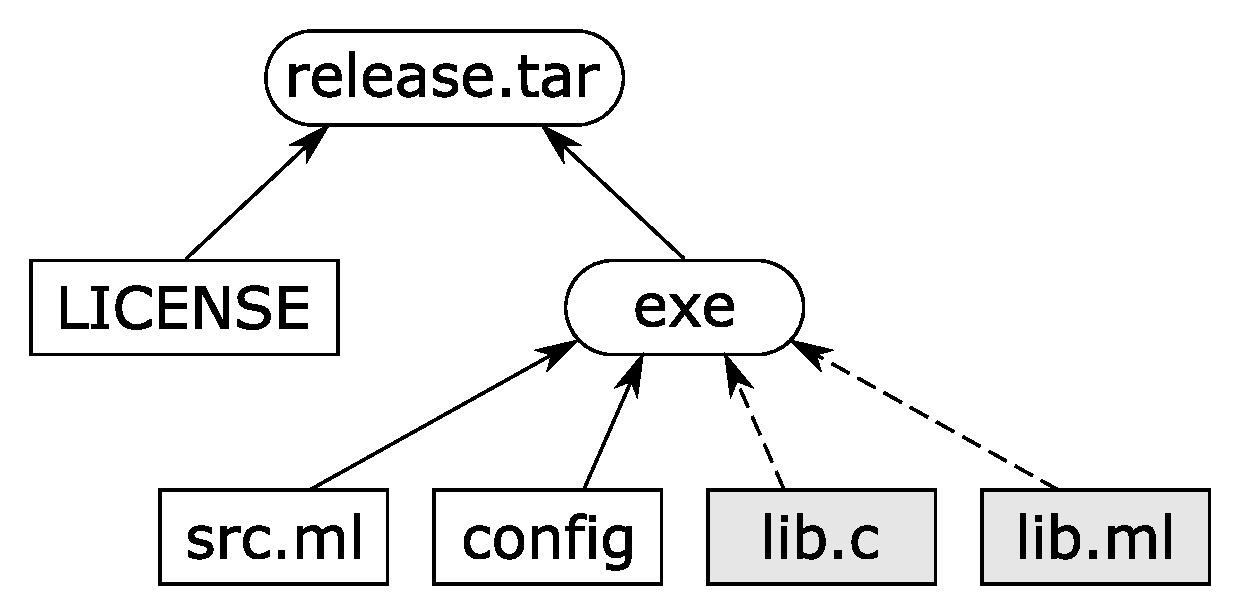
\includegraphics[scale=0.3]{fig/build-dependencies.pdf}}
\vspace{-2mm}
\caption{An example build dependency graph. Input files are shown in rectangles,
intermediate and output files are shown in rounded rectangles. Conditional
dependencies are highlighted with dashed lines.}
\label{fig-build}
\vspace{-4mm}
\end{figure}

By analysing individual build tasks using \hs{dependenciesOver} and
\hs{dependenciesUnder}, we can construct a dependency graph, where some of the
dependencies are conditional, see Fig.~\ref{fig-build}:

\vspace{1mm}
\begin{minted}[xleftmargin=10pt]{haskell}
@\ghci@ dependenciesOver (fromJust $ script "release.tar")
["LICENSE","exe"]
@\ghci@ dependenciesUnder (fromJust $ script "release.tar")
["LICENSE","exe"]
@\ghci@ dependenciesOver (fromJust $ script "exe")
["src.ml","config","lib.c","lib.ml"]
@\ghci@ dependenciesUnder (fromJust $ script "exe")
["src.ml","config"]
\end{minted}
\vspace{1mm}

Note that while over-approximation is useful for installing all possible
dependencies \emph{before the build}, under-approximation is useful for
maximising parallelism \emph{during the build}: for example, if all input files
are actually generated by running a text preprocessor, then we can start the
three preprocessing tasks that are definitely needed (\cmd{LICENSE},
\cmd{src.ml}, \cmd{config}) in parallel, i.e. without waiting for the outcome of
parsing the \cmd{config} file.

\emph{Applicative and monadic build systems} studied in~\citep{mokhov2018build}
cannot support such over- and under-approximating static analysis, and the
associated abstractions are therefore unsuitable for \Dune. This explains why
\Dune developers have chosen to use the \emph{arrow} abstraction
(\S\ref{sec-arrows}). As our case study and the developed prototype demonstrate,
selective functors provide a viable alternative to arrows in the context of
build systems.

% Dune is another example where the extra power provided by selective
% functions is relevant. To understand why, let's consider the following
% example: a user wants to use some optimized C function if it is
% available on the system, and fallback to an OCaml implementation if
% not. The C and OCaml implementations might have different external
% dependencies. Such a test is dynamic since it depends on the system
% the users builds the software on. During compilation, we only want to
% follow one of the branch, as we clearly don't want to build
% implementation only to keep a single one. However, during dependency
% analysis for the project manifest we need to scan both branches. The
% dependencies discovered in both branches will be considered as
% optional dependencies given that neither is always required.

% For parallelism use underapproximation: take intersection of optional
% dependencies, and then union with necessary dependencies.
% Note that this requires 'branch' to be in the type class, so we
% can see both branches and intersect their effects.

\section{Speculative Execution}\label{sec-haxl}

\Haxl~\citep{marlow2014haxl} is a framework for efficiently executing
code that fetches data from external sources, typically databases or
remote services. The \Haxl framework allows code written in a natural
style using \hs{Applicative} and \hs{Monad} combinators to run
efficiently, by automatically parallelising the data fetch operations
and batching together multiple fetches from the same data source.
\Haxl has been in use at Facebook, at scale, for several years now in
a system that proactively detects and remediates various forms of
abuse. \Haxl allows the engineers working on the anti-abuse code to
write clear and concise application logic, because the framework
abstracts away from the details of concurrency and efficient data fetching.

To illustrate the idea using a fragment of the example code
by~\citet{marlow2014haxl}, suppose we are writing the code to render a blog
into HTML. The blog consists of a set of posts, where each post is identified by
a \hs{PostId}. The data for the blog is stored in a remote database, and the API
for fetching the data from the database is as follows:

\vspace{1mm}
\begin{minted}[xleftmargin=10pt]{haskell}
getPostIds     :: Haxl [PostId]
getPostContent :: PostId -> Haxl PostContent
\end{minted}
\vspace{1mm}

\noindent
We can fetch the set of all \hs{PostId}s using \hs{getPostIds}, and we can fetch
the content of one post using \hs{getPostContent}. To get the content of all
posts we could write:

\vspace{0.5mm}
\begin{minted}[xleftmargin=10pt]{haskell}
getAllPostsContent :: Haxl [PostContent]
getAllPostsContent = getPostIds >>= mapM getPostContent
\end{minted}
\vspace{0.5mm}

\noindent
Now, when we \hs{mapM}~\hs{getPostContent} we would really like the
database queries to happen in parallel, because there are no
dependencies between them. Furthermore, we might even be able to batch
up the queries into a single request to the remote database.

\begin{figure}
\begin{minted}[fontsize=\small]{haskell}
-- A Haxl computation is either completed (Done) or Blocked on pending data requests
data Result a = Done a | Blocked BlockedRequests (Haxl a) deriving Functor
newtype Haxl a = Haxl { runHaxl :: IO (Result a) } deriving Functor
\end{minted}
\vspace{0mm}
\begin{minted}[fontsize=\small]{haskell}
instance Applicative Haxl where
  pure = Haxl . return . Done
  Haxl iof <*> Haxl iox = Haxl $ do
    rf <- iof
    rx <- iox
    return $ case (rf, rx) of
      (Done f      , _           ) -> f    <$> rx
      (_           , Done x      ) -> ($x) <$> rf
      (Blocked bf f, Blocked bx x) -> Blocked (bf <> bx) (f <*> x)
\end{minted}
\vspace{-13.5mm}\hspace{95mm}
\includegraphics[scale=0.32]{fig/comment-haxl-applicative.pdf}
\vspace{3mm}
\begin{minted}[fontsize=\small]{haskell}
instance Selective Haxl where
  select (Haxl iox) (Haxl iof) = Haxl $ do
    rx <- iox
    rf <- iof
    return $ case (rx, rf) of
      (Done (Right b), _           ) -> Done b
      (Done (Left  a), _           ) -> ($a) <$> rf
      (_             , Done       f) -> either f id <$> rx
      (Blocked bx x  , Blocked bf f) -> Blocked (bx <> bf) (select x f)
\end{minted}
\vspace{-26mm}\hspace{31.5mm}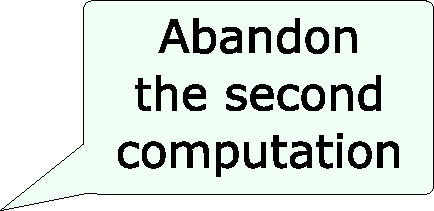
\includegraphics[scale=0.32]{fig/comment-haxl-selective-1.pdf}
\vspace{11.5mm}\hspace{110.5mm}
\includegraphics[scale=0.32]{fig/comment-haxl-selective-2.pdf}
\vspace{-7.5mm}
\begin{minted}[fontsize=\small]{haskell}
instance Monad Haxl where
  return = Haxl . return . Done
  Haxl iox >>= f = Haxl $ do
    rx <- iox
    case rx of Done       x -> runHaxl (f x)
               Blocked bx x -> return (Blocked bx (x >>= f))
\end{minted}
\vspace{-19mm}\hspace{31mm}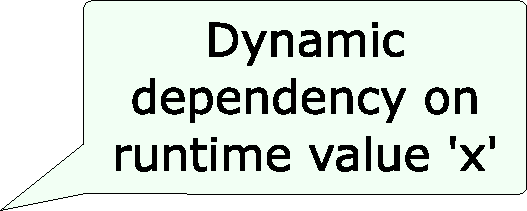
\includegraphics[scale=0.32]{fig/comment-haxl-monad.pdf}
\vspace{5mm}
\caption{An implementation of \hs{Applicative}, \hs{Selective} and \hs{Monad}
instances for the \Haxl monad.}
\label{fig-haxl}
\vspace{-3mm}
\end{figure}

These optimisations are performed automatically by \Haxl, using a
special \hs{Applicative} instance that exploits the lack of
dependency between the two computations to explore the computations
and collect the data fetch requests that can be performed in parallel or batched
together. Fig.~\ref{fig-haxl} shows an implementation adapted from the code
by~\citet{marlow2014haxl}. For the purposes of the presentation here we have
renamed \hs{Fetch} to \hs{Haxl} and omitted the exception-handling code.
The key piece of \Haxl's design is the \hs{Blocked}/\hs{Blocked} case, where
two independent sets of \hs{BlockedRequests} are combined together (the
semigroup operator \hs{<>} is just a customised set union). \Haxl also has a
\hs{Monad} instance, also shown in Fig.~\ref{fig-haxl}, which provides support
for \emph{dynamic} data fetches that are based on results obtained earlier.
Such dynamic data fetches are sequentialised as you would expect, but code
written to use \hs{Applicative} operations benefits from the automatic
concurrency. This optimisation is further exploited by using a transformation
on the monadic \cmd{do}-notation to automatically use \hs{Applicative}
operators where possible~\cite{marlow2016applicativedo}.

One of the key tools found to be useful in the kind of code written
using \Haxl at Facebook is the ``lazy'' conditional operators:

\vspace{1mm}
\begin{minted}[xleftmargin=10pt]{haskell}
(.||), (.&&) :: Haxl Bool -> Haxl Bool -> Haxl Bool
@\blk{x}@ .|| y = do b <- x; if b then return True else y
@\blk{x}@ .&& y = do b <- x; if b then y           else return False
\end{minted}
\vspace{1mm}

\noindent
These are typically used to improve performance by guarding slow
checks with faster checks.  For example, we might write:

\begin{minted}[xleftmargin=10pt]{haskell}
if simpleCondition .&& complexCondition then ... else ...
\end{minted}

\noindent
The idea is that \hs{simpleCondition} is quick to evaluate and
returns \hs{False} in a large proportion of cases, so that we can
often avoid needing to evaluate \hs{complexCondition}.

This does not require any additional extensions or special support in
\Haxl. But we also noticed that sometimes there is a pair of conditions
where neither is obviously faster than the other, yet we would still
like to benefit from bailing out early when the answer is known.
Therefore, \Haxl contains two more conditional operators \hs{pOr} and
\hs{pAnd} for ``parallel OR'' and ``parallel AND'':

\begin{minted}[xleftmargin=10pt]{haskell}
pOr, @\blu{pAnd}@ :: Haxl Bool -> Haxl Bool -> Haxl Bool
\end{minted}

\noindent
These have the behaviour that: (i)~both arguments are evaluated in parallel;
(ii)~the computation is aborted as soon as the answer is known, even if the
other argument is still being evaluated. Data fetches are not observable
effects, so the parallelism is not observable to the programmer (\Haxl relies
on this property for the soundness of its parallel \hs{Applicative}
instance). However, \hs{pOr} and \hs{pAnd} are non-deterministic with
respect to exceptions: if an exception is thrown by either side, it
will be thrown by the computation as a whole immediately without
waiting for the other side to complete.  One could imagine an
alternative implementation which waits for the completion of the other
argument when an exception is raised; this would be deterministic, but
would be less efficient in the case of exceptions.

It should come as no surprise that \hs{pOr} and \hs{pAnd} can be
implemented using \hs{select}, indeed \hs{pOr}~\hs{=}~\hs{(<||>)} and
\hs{pAnd}~\hs{=}~\hs{(<&&>)} from Fig.~\ref{fig-library}. The corresponding
\hs{Selective} instance is given in Fig.~\ref{fig-haxl}: in the
\hs{Blocked}/\hs{Blocked} case we speculatively explore both computations,
and if we obtain a \hs{Done}/\hs{Right} result, the second computation is
safely abandoned and subsequently cancelled.

There is one wrinkle with implementing \hs{pOr} and \hs{pAnd}
in terms of \hs{select}. Ideally, \hs{pOr} and \hs{pAnd} would be
symmetric: just as we can cancel the second computation if the first
one determines the answer, we should be able to cancel the first
computation in the same way. Yet \hs{select} is inherently left-biased:
it requires that all the effects of the first argument are performed.
In~\S\ref{sec-alt-symmetric} we consider an alternative combinator
related to \hs{select} that allows this kind of symmetry to be expressed.

We have prototyped an implementation of \Haxl with the \hs{Selective}~\hs{Haxl}
instance, which allowed us to reuse generic selective combinators
\hs{<||>}, \hs{<&&>}, \hs{anyS} and \hs{allS} instead of providing custom
implementations for conditional operators \hs{pOr} and \hs{pAnd} and
their generalisations on lists. This case study highlights the fact that
selective functors are useful not only in the static context, but in the dynamic
context too, by allowing us to benefit from speculative execution.

\subsection{Results}

We mentioned above that \hs{pOr} and \hs{pAnd} are effective when the
relative size of the conditional computations is unknown, so
evaluating them in parallel with early exit is an effective
alternative to either sequencing them manually (with \hs{Monad}) or
evaluating them in parallel to completion (with
\hs{Applicative}). This argument becomes even more compelling as the
set of conditions to evaluate grows: imagine trying to efficiently
sequence a set of ten or more conditions, and then repeating the
exercise every time the set changes.

For this reason, in \Haxl we found that list operations built on top
of \hs{pOr} and \hs{pAnd}, which in this paper we call \hs{anyS} and
\hs{allS} (see Fig.~\ref{fig-library}), offer an important balance
between performance and maintainability that is not provided by the
\hs{Applicative} or \hs{Monad}-based combinators.

One could construct examples to demonstrate arbitrarily large
performance gains from using \hs{pOr} and \hs{pAnd}, however that
would not be particularly useful. Perhaps more useful would be a
real-world measurement showing how much performance was improved in an
actual application but again, the value of that would depend to a
large extent on how the application uses \hs{pOr} and \hs{pAnd}, and
unfortunately the application code in our case is
proprietary. Therefore instead we offer this anecdote: we first
introduced a use of \hs{pOr} to solve some performance issues in a
complex production workload where we had long chains of conditionals
that were difficult to optimise by hand, and \hs{pOr} resulted in
significant performance improvements.

\section{Free Selective Functors}\label{sec-free}

The idea of describing effectful computations using \emph{free constructions},
such as \emph{free}~\cite{swierstra2008data} and \emph{freer
monads}~\cite{kiselyov2015freer} and \emph{free applicative
functors}~\cite{free-applicatives} is well-studied in the functional programming
community. Free constructions allow us to focus on the internal aspects of the
effect under consideration and receive the desired applicative or monadic
computation structure \emph{for free}, i.e. without the need to define custom
instances or prove laws.

In this section we apply this idea to selective functors. We present a free
construction for \emph{rigid} selective functors
(\S\ref{sec-free-construction}), and demonstrate it on two examples
in~\S\ref{sec-free-ping-pong} and~\S\ref{sec-free-isa}.

\subsection{Free Construction}\label{sec-free-construction}

In the free structures methodology, the essence of an effect is captured by a
data type that encodes the ``commands'' which the effect provides, acting as a
deep embedding of the effect's interface. This data type needs only have enough
structure to be a~\hs{Functor}. The purpose of a free construction is then to
build a richer structure on top of this \emph{base functor}, which would have
the desired instances, in our case \hs{Applicative} and \hs{Selective}. In this
section we will denote the base functor by \hs{f}.

\begin{figure}
\begin{minted}[fontsize=\small]{haskell}
data Select f a where
    Pure   :: a -> Select f a
    Select :: Select f (Either a b) -> f (a -> b) -> Select f b
\end{minted}
\vspace{0mm}
\begin{minted}[fontsize=\small]{haskell}
instance Functor f => Functor (Select f) where
    fmap f (Pure a)     = Pure (f a)
    fmap f (Select x y) = Select (fmap f <$> x) (fmap f <$> y) -- Free theorem from Fig. 4
\end{minted}
\vspace{0mm}
\begin{minted}[fontsize=\small]{haskell}
instance Functor f => Applicative (Select f) where
    pure  = Pure
    (<*>) = apS -- Law of rigid selective functors
\end{minted}
\vspace{0mm}
\begin{minted}[fontsize=\small]{haskell}
instance Functor f => Selective (Select f) where
    select x (Pure y)     = either y id <$> x -- Generalised identity
    select x (Select y z) = Select (select (f <$> x) (g <$> y)) (h <$> z) -- Associativity
      where
        f x = Right <$> x
        g y = \a -> bimap (,a) ($a) y
        h z = uncurry z
\end{minted}
\vspace{0mm}
\begin{minted}[fontsize=\small]{haskell}
-- Lift a base functor into Select
liftSelect :: Functor f => f a -> Select f a
liftSelect f = Select (Pure (Left ())) (const <$> f)
\end{minted}
\vspace{0mm}
\begin{minted}[fontsize=\small]{haskell}
-- Interpret a free selective structure given a natural transformation from f to g
runSelect :: Selective g => (forall x. f x -> g x) -> Select f a -> g a
runSelect _ (Pure a)     = pure a
runSelect t (Select x y) = select (runSelect t x) (t y)
\end{minted}
\vspace{0mm}
\begin{minted}[fontsize=\small]{haskell}
-- Extract the resulting value from a pure selective computation
getPure :: Select f a -> Maybe a
getPure = runSelect (const Nothing)
\end{minted}
\vspace{0mm}
\begin{minted}[fontsize=\small]{haskell}
-- Extract all possible effects from a selective computation
getEffects :: Functor f => Select f a -> [f ()]
getEffects = getOver . runSelect (Over . pure . void)
\end{minted}
\vspace{-3mm}
\caption{A basic implementation of free rigid selective functors; various
improvements are omitted for clarity.}\label{fig-free}
\vspace{-3mm}
\end{figure}

As we remarked in~\S\ref{sec-laws}, rigid selective functors have a particularly
simple normal form thanks to the additional law \hs{(<*>)}~\hs{=}~\hs{apS},
which tells us that the apply operator \hs{<*>} is redundant and can be
implemented via the selective interface. This normal form has the following
linear structure:

\vspace{1mm}
\begin{minted}[xleftmargin=10pt]{haskell}
pure x <*? fa <*? fb <*? ... <*? fy
  where
    x  :: Either a (Either b (Either c (... z)))
    fa :: f (a ->   Either b (Either c (... z)))
    fb :: f (b ->             Either c (... z))
    ...
    fy :: f (y ->                           z)
\end{minted}
\vspace{1mm}

\noindent
In words, any rigid selective computation can be rewritten as a left-associated
sequence of select operators, where the initial pure value~\hs{x} belongs to a
large sum type (comprising alternatives~\hs{a}~to~\hs{z} in the above snippet),
and each of the subsequent effects eliminates one of the alternatives, in order,
until only one remains (namely, \hs{z}).

Interestingly, there is no right-associated version of the normal form because
the associativity law~(\S\ref{sec-laws}) can only be used to re-associate an
expression to the left, which is a consequence of the asymmetry of the select
operator. It is worth noting that this is different from applicative functors
that have two normal forms corresponding to left and right
re-association of the apply operator~\citep{free-applicatives}. A symmetric
version of the select operator, which can be re-associated in either direction,
is discussed in~\S\ref{sec-alt-symmetric}.

% To apply it in reverse, we would need to ``factor out'' the reshaping functions
% \hs{f}, \hs{g} and \hs{h} from the base functor, which is not always possible.

% To see why, consider the expression
% \hs{pure}~\hs{(Right}~\hs{(Left}~\hs{1))}~\hs{<*?}~\hs{p}~\hs{<*?}~\hs{q}, where
% the effect \hs{p} is unnecessary due to the leading selector \hs{Right}. It is
% not possible to re-associate this expression into
% \hs{pure}~\hs{(Right}~\hs{(Left}~\hs{1))}~\hs{<*?}~\hs{(@@p'}~\hs{<*?}~\hs{q')}
% because in the sub-expression \hs{(@@p'}~\hs{<*?}~\hs{q')} the first effect
% \hs{p'} cannot be skipped.

Fig.~\ref{fig-free} gives an encoding of this normal form in Haskell. The free
data type \hs{Select} represents a selective computation as a type-aligned
sequence of base functor effects, with the \hs{Pure} constructor at the head.
Instance definitions rely on the selective laws from~\S\ref{sec-laws},
specifically: generalised identity, associativity, and one of the free theorems.
We do not use distributivity as it is subsumed by the law of rigid selective
functors \hs{(<*>)}~\hs{=}~\hs{apS}, used in the \hs{Applicative} instance.

Effects of the base functor can be embedded in the free construction using
the helper function \hs{liftSelect}. To interpret a free selective computation
\hs{Select}~\hs{f}~\hs{a} in a selective functor \hs{g}, one needs to provide
a \emph{natural transformation} from \hs{f} to \hs{g} to the function
\hs{runSelect}, which traverses the sequence of effects, converts them to
\hs{g}, and composes the results using \hs{g}'s select operator.

For example, \hs{getPure} reinterprets a given free computation in the selective
functor \hs{g}~\hs{=}~\hs{Maybe} using the natural transformation
\hs{const}~\hs{Nothing}, which leaves the \hs{Pure} head of the sequence as is,
but turns any subsequent effect into \hs{Nothing}. Similarly, \hs{getEffects}
records all effects by stashing them in the selective functor \hs{Over}, which
are subsequently extracted from it by \hs{getOver}.

We can improve the encoding in~Fig.~\ref{fig-free} in several ways: (i)~make it
``freer'' by not requiring~\hs{f}~to be a~\hs{Functor}; (ii)~make \hs{fmap} and
\hs{select} asymptotically faster using the ideas
by~\citet{menendez2013free}; and (iii)~drop the rigidity requirement,
obtaining a general free construction for selective functors~---~see an
implementation in the library~\citep{selective2019haskell} and the supplementary
material.

\subsection{Ping-pong, Freely}\label{sec-free-ping-pong}

To illustrate the usage of free selective functors on a simple example, we
implement the classic \cmd{Teletype} DSL~\cite{swierstra2008data} comprising
two commands: \emph{reading} a string form the input stream and \emph{writing}
a string to the output stream. The base functor has two corresponding
constructors:

\vspace{1mm}
\begin{minted}[xleftmargin=10pt]{haskell}
data Teletype a = Read (String -> a) | Write String a deriving Functor
\end{minted}
\vspace{1mm}

\noindent
For convenience, we can provide the following functions that embed the commands
into the free selective construction, mimicking Haskell's \hs{IO} API:

\vspace{1mm}
\begin{minted}[xleftmargin=10pt]{haskell}
getLine :: Select Teletype String
getLine = liftSelect (Read id)
\end{minted}
\vspace{0mm}
\begin{minted}[xleftmargin=10pt]{haskell}
putStrLn :: String -> Select Teletype ()
putStrLn s = liftSelect (Write s ())
\end{minted}
\vspace{1mm}

\noindent
We can now reimplement the \hs{pingPongS} example from~\S\ref{sec-intro} in
terms of the free selective construction simply by adjusting the type signature.
Note that the \hs{whenS} combinator comes for free.

\vspace{1mm}
\begin{minted}[xleftmargin=10pt]{haskell}
pingPongS :: Select Teletype ()
pingPongS = whenS (fmap (=="ping") getLine) (putStrLn "pong")
\end{minted}
\vspace{1mm}

\noindent
By embedding \hs{pingPongS} into the free construction, we gain access to the
static analysis machinery:

\vspace{1mm}
\begin{minted}[xleftmargin=10pt]{haskell}
@\ghci@ getEffects pingPongS
[Read,Write "pong"]
\end{minted}
\vspace{1mm}

\noindent
The function \hs{getEffects} (Fig.~\ref{fig-free}) returns the list of all
effects of a free selective computation. In the case of \cmd{Teletype},
we get a list of all \hs{Read}/\hs{Write} commands that a computation might
execute.

We can interpret \cmd{Teletype} programs in any other selective functor using
the \hs{runSelect} function by providing a natural transformation
\hs{forall}~\hs{x.}~\hs{Teletype}~\hs{x}~\hs{->}~\hs{g}~\hs{x}, which assigns an
interpretation to \cmd{Teletype} commands in terms of \hs{g}. A good example of
such transformation would be an interpretation in the \hs{IO} monad, which
allows us to execute our \hs{pingPongS} program:

\vspace{1mm}
\begin{minted}[xleftmargin=10pt]{haskell}
toIO :: Teletype a -> IO a
toIO (Read f)    = f <$> Prelude.getLine
toIO (Write s a) = a <$  Prelude.putStrLn s
\end{minted}
\vspace{0mm}
\begin{minted}[xleftmargin=10pt]{haskell}
@\ghci@ runSelect toIO pingPongS
hello
@\ghci@ runSelect toIO pingPongS
ping
pong
\end{minted}
\vspace{1mm}

\noindent
Note that while we can write simple programs like \hs{pingPongS} using the
selective interface, we are fundamentally limited in what we can express
compared to the much more powerful monadic interface. As an example, consider
this simple greeting program:

\vspace{1mm}
\begin{minted}[xleftmargin=10pt]{haskell}
greeting = getLine >>= \name -> putStrLn ("Hello " ++ name)
\end{minted}
\vspace{1mm}

\noindent
Programs like this cannot be expressed in our simple \cmd{Teletype} DSL. Even if
we had \hs{bindS} for strings~(\S\ref{sec-alt-multi}), it would be useless for
static analysis because it would have to report effects \hs{Write}~\hs{s} for
\emph{all possible strings} \hs{s}! Nevertheless, limitations of the selective
interface can sometimes be worked around by using more sophisticated base
functors, as we show in~\S\ref{sec-free-isa}.

% Software build systems can be modelled with purely functional
% abstractions~\cite{mokhov2018build} that enable the model to accommodate many
% different build systems and express their features in a way that allow for deriving
% new build systems by combining the best parts of the existing ones. The approach
% presented on~\cite{mokhov2018build} allows to distinguish the \emph{static} build
% dependencies from the \emph{dynamic} ones by expressing the build tasks which
% may only have static dependencies with the \hs{Applicative} interface, and using
% \hs{Monad} for constructing build tasks with dynamic dependencies.
% As selective functors give us the best of both worlds, we show how we could adopt
% their free construction to build a deep embedding of the \hs{fetch} callback from
% the original paper.

% To use any free construction, we need to invent an underlying functor, which would
% be the essence of the effect we are trying to implement. In case of the \hs{fetch}
% callback, we require an effect of a read-only store:

% \begin{minted}[xleftmargin=10pt]{haskell}
% data Fetch k v a = Fetch k (v -> a)
%    deriving Functor
% \end{minted}

% That is, the \hs{Fetch} functor has only one data constructor, which represents a
% command with a suggested semantics of extracting a value associated with a key from
% the store.

% We cannot directly use the \hs{Fetch} command in a selective computations, thus we
% embed it into a free selective construction by simply lifting the data constructor
% in the following way:

% \begin{minted}[xleftmargin=10pt]{haskell}
% fetch :: k -> Select (F k v) v
% fetch key = liftSelect $ Fetch key id
% \end{minted}

\subsection{Analysis and Simulation of Processor Instructions}\label{sec-free-isa}

To demonstrate the free construction on a more interesting example, we apply it
to analysis and simulation of a hypothetical instruction set architecture
(ISA)\footnote{Incidentally, this was the original motivation for selective
functors. While describing the formal semantics of instructions of a real
processor, we needed a statically analysable \hs{ifS} for the purpose of
symbolic program verification, which eventually led us to \hs{select}. We use a
hypothetical ISA in this section instead of the real one, because of the
complexity of the latter.}. By expressing the ISA semantics in our
free construction with an unusual base functor, we will be able to build
tools both for static data flow analysis and simulation of programs with
branching.

\vspace{-1mm}
\subsubsection{ISA Semantics}
To work around some of the aforementioned limitations of the selective
interface (namely, the lack of the bind operator), we represent the semantics of
instructions thus:

\vspace{1mm}
\begin{minted}[xleftmargin=10pt]{haskell}
type Program a = Select RW a
\end{minted}
\vspace{-0.5mm}
\begin{minted}[xleftmargin=10pt]{haskell}
data RW a = Read  Key                 (Value -> a)
          | Write Key (Program Value) (Value -> a) deriving Functor
\end{minted}
\vspace{1mm}

\noindent
The \hs{RW} (pronounced ``read-write'') base functor encodes the effect of a
mutable key-value store comprising two commands: (i)~we need the ability to
\emph{read} a value associated with a key from the store, and (ii) given a
computation which produces a value, \emph{write} its result into the store.
Think of \hs{Value} as a machine word, and \hs{Key} as an ISA memory location
(a register, a memory cell, or a processor flag). The base commands are similar
to \cmd{Teletype}, with one key difference: the \hs{Write} constructor takes
\hs{Program}~\hs{Value}, i.e. a computation producing a value instead of just
plain \hs{Value}.

This exact structure of the definition is required for accommodating a pattern
that occurs frequently in instruction semantics: often we read a value from a
register or a memory cell, do something with it, and then write it somewhere
else. If \hs{Write} required the second argument to be a pure value, as in
\cmd{Teletype}, we would not be able to express the desired pattern without
resorting to the monadic interface. Additionally, we want the \hs{Write}
command to not just write the value and return \hs{()}, but to \emph{give the
just written value back}, so it can be used in the rest of the computation; such
generosity of the \hs{Write} command will be useful for avoiding duplicate data
dependencies.

We introduce two convenience combinators, which lift the data constructors of
the \hs{RW} data type into the free selective, thus making them directly usable
in the definitions of instruction semantics:

\vspace{1mm}
\begin{minted}[xleftmargin=10pt]{haskell}
read :: Key -> Program Value
read k = liftSelect (Read k id)
\end{minted}
\vspace{-0.5mm}
\begin{minted}[xleftmargin=10pt]{haskell}
write :: Key -> Program Value -> Program Value
write k fv = liftSelect (Write k fv id)
\end{minted}
\vspace{1mm}

\vspace{-1mm}
\subsubsection{Example 1. Addition}
To get acquainted with the introduced vocabulary, we start by describing the
semantics for the addition instruction, which reads the summands from a
register and a memory cell, adds them, writes the result back into the same
register, and also updates the state of the \hs{Zero} flag to indicate whether
the resulting value is zero.

\vspace{1mm}
\begin{minted}[xleftmargin=10pt]{haskell}
add :: Register -> Address -> Program Value
add reg addr = let arg1   = read (Reg reg)
                   arg2   = read (Cell addr)
                   result = (+)   <$> arg1 <*> arg2
                   isZero = (==0) <$> write (Reg reg) result
               in write (Flag Zero) (bool 0 1 <$> isZero)
\end{minted}
\vspace{1mm}

\noindent
Here, we \hs{read} the summands \hs{arg1} and \hs{arg2} from the two specified
locations and calculate the \hs{result} of addition by lifting \hs{(+)} into the
free selective functor using applicative combinators. We then calculate the
value of the \hs{Zero} flag in a similar way, but here we exploit the fact that
the \hs{write} combinator returns the value it has just written, thus we can
reuse the \hs{result} without recalculating it from scratch (which would
duplicate the corresponding read effects).

By analysing the free semantics of the \hs{add} instruction, we can obtain the
list of all its effects, in the order they appear in the computation. We also
visualise the effects as a data flow graph, where data locations are shown as
rectangles, instructions as rounded rectangles, and reads/writes as arcs.

% \footnote{For didactic purposes,
% these graph was hand-crafted, but it is possible to get similar results
% automatically with Graphviz~\cite{ellson2001graphviz}.}

\begin{figure}[!h]
\begin{minipage}{0.53\textwidth}
\raggedleft
\begin{minted}[xleftmargin=10pt]{haskell}
@\ghci@ getProgramEffects (add R0 1)
[Read R0,Read 1,Write R0,Write Zero]
\end{minted}
 \end{minipage}
 \begin{minipage}{0.44\textwidth}
  \centering
  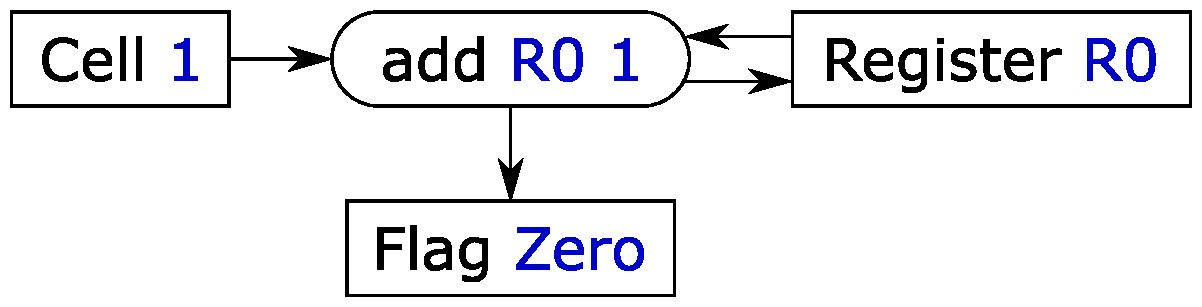
\includegraphics[scale=0.3]{fig/add.pdf}
 \end{minipage}
\end{figure}

\noindent
To implement \hs{getProgramEffects}, we apply the natural transformation
\hs{toOver} to the effects of a \hs{Program}, which recursively collects the
effects that occur in the \hs{Write}'s argument \hs{fv}:

\vspace{1mm}
\begin{minted}[xleftmargin=10pt]{haskell}
getProgramEffects :: Program a -> [RW ()]
getProgramEffects = getOver . runSelect toOver
\end{minted}
\vspace{1mm}
\begin{minted}[xleftmargin=10pt]{haskell}
toOver :: RW a -> Over [RW ()] a
toOver (Read  k _   ) = Over [Read k (const ())]
toOver (Write k fv _) = runSelect toOver fv *> Over [Write k fv (const ())]
\end{minted}
\vspace{1mm}

\noindent
The semantics of the addition instruction has only used applicative combinators
and we thus could have analysed it statically using free applicative functors.
However, there are important instructions whose semantics cannot be expressed
in terms of the \hs{Applicative} interface, and this is where the presented
free selective construction becomes irreplaceable.

\subsubsection{Example 2. Conditional Jump}

Selective functors introduce limited dependencies between effectful
computations, giving us enough power to express the semantics of branching
instructions, which modify the program counter by a given offset if a certain
condition holds. Consider the following instruction that performs a jump if the
result of the previous operation was zero.

\vspace{1mm}
\begin{minted}[xleftmargin=10pt]{haskell}
jumpZero :: Value -> Program ()
jumpZero offset = let zeroSet  = (==1) <$> read (Flag Zero)
                      modifyPC = void $ write PC ((+offset) <$> read PC)
                  in whenS zeroSet modifyPC
\end{minted}
\vspace{1mm}

\noindent
Here we use the \hs{whenS} combinator to modify the program counter only if
the \hs{Zero} flag is set. By implementing \hs{jumpZero} in terms of the
selective interface, we achieve both the ability to implement an adequate
simulator for branching programs and perform their static analysis:

\vspace{1mm}
\begin{figure}[!h]
 \begin{minipage}{0.45\textwidth}
\raggedleft
\begin{minted}[xleftmargin=7pt]{haskell}
@\ghci@ getProgramEffects (jumpZero 42)
[Read Zero,Read PC,Write PC]
\end{minted}
 \end{minipage}
 \begin{minipage}{0.54\textwidth}
  \centering
  
\includegraphics[scale=0.3]{fig/jumpZero.pdf}
 \end{minipage}
\end{figure}
\vspace{1mm}

\noindent
Since the analysis is static, the resulting list of effects and the
corresponding data flow graph are over-approximations and show all effects that
can possibly happen during the execution.

% Note that it does not matter which argument we supply to \hs{jumpZero}, since
% it will never get forced, e.g. the analysis will succeed and give us the same
% result even if we supply \hs{undefined}.

\subsubsection{Example 3. Blocks of Instructions}

Once we have implemented the semantics for a desired subset of an ISA, we can
describe the semantics of sequences, or \emph{blocks}, of instructions by
simply composing the semantics of individual instructions using the applicative
sequencing operator (\hs{*>}):

% \vspace{1mm}
\begin{minted}[xleftmargin=10pt]{haskell}
addAndJump :: Program ()
addAndJump = add R0 1 *> jumpZero 42
\end{minted}
\vspace{1mm}

\noindent
We can analyse such compound computations in the same way as we analyse
individual instructions:

\vspace{-1mm}
\begin{figure}[!h]
 \begin{minipage}{0.46\textwidth}
\raggedleft
\begin{minted}{haskell}
@\ghci@ getProgramEffects addAndJump
[Read R0,Read 1,Write R0,Write Zero
,Read Zero,Read PC,Write PC]
\end{minted}
 \end{minipage}
 \begin{minipage}{0.50\textwidth}
  \centering
  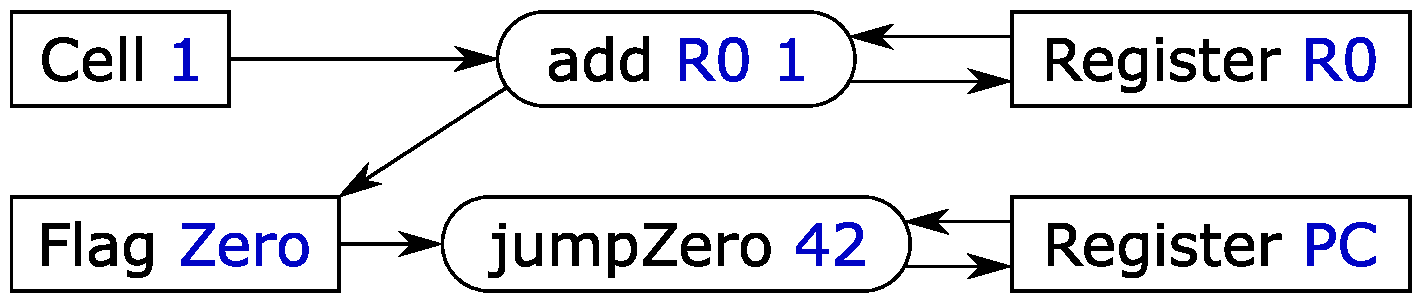
\includegraphics[scale=0.3]{fig/addAndJump.pdf}
 \end{minipage}
\end{figure}
\vspace{-1mm}

% Getting a flat list of effects that blocks of code perform is not very useful,
% since they does not carry any explicit data-flow information. To mitigate this
% restriction, we take the following approach. We create a (1) deeply-embedded
% assembly language and (2) implement an interpreter which assigns a semantics to
% this language in terms of the free selective construction. By doing this, we can
% then implement a mechanical procedure which would construct \emph{data flow
% graphs} of sequences of instructions, similar to the ones shown in
% Fig.~\ref{fig-addAndJump-gcd} by overlaying the graphs for single instructions.
% Note that if an instruction performs multiple read/writes of the same location,
% we will deliberately merge them in the resulting graph.

\subsubsection{Simulation}

To implement an ISA simulator, we follow the same path as in the \hs{pingPongS}
example and the \hs{IO} monad earlier in~\S\ref{sec-free-ping-pong}. We need a
natural transformation from the base functor \hs{RW} to an appropriate target
functor, e.g. an instance of \hs{MonadState}~\hs{ISAState}, where \hs{ISAState}
represents the state of all registers, memory cells and flags. For brevity, we
present only one part of such a transformation, which assigns an interpretation
to reading and writing of register keys~\hs{Reg}:

\vspace{1mm}
\begin{minted}[xleftmargin=10pt]{haskell}
toState :: MonadState ISAState m => RW a -> m a
toState (Read k t) = t <$> case k of
    Reg r -> (Map.! r) <$> gets registers -- Look up r in the registers field
    ...
toState (Write k fv t) = case k of
    Reg r -> do v <- runSelect toState fv -- Evaluate the Write's argument
                let step s = Map.insert r v (registers s)
                state $ \s -> (t v, s { registers = step s })
    ...
\end{minted}
\vspace{1mm}

\noindent
To read a register, we simply lift the lookup function \hs{Map.!} to the
corresponding field of the \hs{ISAState}. To write an effectful value \hs{fv}
into a register, we need to evaluate it first; hence we call the \hs{runSelect}
function, supplying it the natural transformation \hs{toState}, recursively,
thus performing the effects of \hs{fv}. We then adjust the register bank with
the new value and return it.

The natural transformation \hs{toState} gives interpretation to individual
\hs{Read} and \hs{Write} commands, and now this interpretation can be extended
to any \hs{Program} by plugging it into a \hs{runSelect} call, as has already
been done once in the implementation of \hs{toState} itself:

\vspace{1mm}
\begin{minted}[xleftmargin=10pt]{haskell}
runProgram :: Program a -> ISAState -> (a, ISAState)
runProgram p = runState (runSelect toState p)
\end{minted}

\subsubsection{Limitations}

The free selective construction in combination with the base functor \hs{RW}
provides an abstraction capable of expressing the semantics of arithmetic,
load/store and branching instructions. However, one should remember that
selective functors still lack the full expressive power of the monadic interface
and are unable to accommodate an important class of instructions, specifically
those that use the \emph{memory-indirect addressing mode}. If we had a
\hs{Monad}~\hs{Program} instance, we could give the following semantics to the
memory-indirect load instruction \hs{loadMI}:

\vspace{1mm}
\begin{minted}[xleftmargin=10pt]{haskell}
loadMI :: Register -> Address -> Program Value
loadMI reg addr = read (Cell addr) >>= \x -> write (Reg reg) (read (Cell x))
\end{minted}
\vspace{1mm}

\noindent
Here, we read from a memory cell \hs{addr}, then use the monadic bind operator
to extract a value~\hs{x} from the result, and use it in a subsequent memory
read \emph{as address}. Although this semantics is, in principle, implementable
using the selective \hs{bindS} combinator (see \S\ref{sec-alt-multi}), it is not
very useful in practice since static analysis would record possible access to
\emph{all memory cells}~\hs{x}, and there are too many of them (typically, a
large power of two). Furthermore, the execution of the resulting semantics would
be terribly slow, since it would also follow the same linear exploration of the
memory address space (although see \S\ref{sec-alt-multi} for a possible solution
of the performance issue).

% not get any strong benefits. Specifically, since the \hs{getProgramEffects} function,
% which performs static analysis of effects, constructs a conservative
% over-approximation, it would always report something similar to this:
% \hs{[Read addr,Write reg, Write reg...}, which would contain as much instances
% of the \hs{Write} effects as much inhabitants there are in the address
% datatype (usually a large power of two).  Therefore, we lose static analysis.
% Maybe we could get some benefit in simulation? No, unfortunately we, again,
% will not, since \hs{bindS} cannot get magically translated to the monadic
% \hs{>>=}, but instead performs explicit enumeration of inhabitants of the
% bound variable's type, which causes terrible performance regression comparing
% to a monadic implementation. Considering these arguments, using \hs{bindS} for
% mimicking monadic behaviour is not feasible in our case and memory-indirect
% load cannot be modelled in by means of the \hs{ISA} datatype.

\section{Alternative Formulations for Selective Functors}
\label{sec-alternatives}

This section discusses alternative versions of the \hs{Selective} type class
that are based on different \hs{select} operators: specifically, the
multi-way~(\S\ref{sec-alt-multi}) and symmetric~(\S\ref{sec-alt-symmetric})
generalisations of \hs{select}, as well as operators that are equivalent to
\hs{select} but may be more convenient to use~(\S\ref{sec-alt-equivalent}). All
of these ideas can be readily integrated into the presented definition of the
\hs{Selective} type class by extending it with new methods and adding new laws
that ensure that the new methods interact with \hs{select} in an appropriate
manner. This is common in standard Haskell libraries, where type classes
\hs{Applicative} and \hs{Monad} include methods like \hs{*>} and \hs{>>} for
performance reasons.

Another alternative, which is worth a remark, is to simply add \hs{select} to
the \hs{Applicative} type class, with the default implementation
\hs{select}~\hs{=}~\hs{selectA}. While this works for the purposes discussed in
this paper, it would make it harder to reason about code with the
\hs{Applicative}~\hs{f} constraint, since the \hs{select} method makes it
possible for effects to depend on values; declaring such a significant ability
by the \hs{Selective}~\hs{f} constraint is arguably a more prudent approach.

\subsection{Multiway Selective Functors}\label{sec-alt-multi}

As mentioned in~\S\ref{sec-selective}, \hs{branch} is a strong contender to be
the main method of the \hs{Selective} type class; it is parametric and all
selective combinators, including \hs{select} itself, can be derived from it:

\vspace{1mm}
\begin{minted}[xleftmargin=10pt]{haskell}
branch :: Selective f => f (Either a b) -> f (a -> c) -> f (b -> c) -> f c
\end{minted}
\vspace{0mm}
\begin{minted}[xleftmargin=10pt]{haskell}
selectB :: Selective f => f (Either a b) -> f (a -> b) -> f b
selectB x y = branch x y (pure id)
\end{minted}
\vspace{1mm}

\noindent
While we prefer \hs{select} for its simplicity, \hs{branch} does provide an
interesting advantage in the context of static analysis. Specifically, it makes
it statically apparent that the two branches are \emph{mutually exclusive}. When
\hs{branch} is ``desugared'' into a sequence of two \hs{select} operations, the
information about the mutual exclusion between the two branches is lost, which
rules out some static analysis scenarios. For example, it may be useful to know
that in our build systems example in~\S\ref{sec-static-example} we never depend
on both \cmd{lib.c} and \cmd{lib.ml}.

Another point in favour of \hs{branch} is performance: the \hs{select}-based
implementation of the \hs{ifS} combinator checks for the \hs{Left} and
\hs{Right} cases in sequence, instead of directly jumping to the correct case,
so a \hs{branch}-based implementation would be more efficient. Furthermore,
$N$-way generalisations of \hs{select} are possible, although the design space
here is quite large. As an example, one might consider adding \hs{bindS} to the
\hs{Selective} type class, i.e. a special case of the monadic bind operator that
is applicable only to enumerable types:

\vspace{1mm}
\begin{minted}[xleftmargin=10pt]{haskell}
bindS :: Selective f => (Bounded a, Enum a, Eq a) => f a -> (a -> f b) -> f b
\end{minted}
\vspace{1mm}

\noindent
The default implementation could be based on sequentially checking for every
possible value using \hs{select}, but monadic instances would supply a much
faster implementation, namely \hs{bindS}~\hs{=}~\hs{(>>=)}. This would allow
static analysis instances to record all possible cases, without incurring
the $O(N)$ slowdown during the execution of an $N$-way branch.

Interestingly, adding the ability to branch on infinite number of cases makes
selective functors equivalent to monads, e.g. see~\citet{peebles2019sigma}.
However, it is worth pointing out that static analysis of such
infinitely-branching selective functors might take infinite time too.

Exploring the design space for ``multiway selective functors'', and using them
for efficient translation of Haskell's \cmd{do}-notation into selective
combinators in the spirit of the \cmd{ApplicativeDo}
extension~\citep{marlow2016applicativedo} is left for future research. For now,
we believe that adding \hs{branch} and/or an equivalent of \hs{bindS} to the
\hs{Selective} type class would be beneficial for performance-sensitive
applications.

\subsection{Symmetric Selective Functors}\label{sec-alt-symmetric}

In this section we address the asymmetry of \hs{select}, which we remarked on
in~\S\ref{sec-haxl} and~\S\ref{sec-free}. The asymmetry can be seen in the fact
that the first argument of \hs{select} must always be executed, while the second
argument may sometimes be skipped. Consider a more symmetric alternative:

\vspace{1mm}
\begin{minted}[xleftmargin=5pt]{haskell}
biselect :: Selective f => f@\,@(Either a b) -> f@\,@(Either a c) -> f@\,@(Either a (b,c))
\end{minted}
\vspace{1mm}

\noindent
This definition is pleasantly symmetric: if either of the arguments yields a
\hs{Left}~\hs{a} value, the other argument \emph{may be skipped} since the
result must be a \hs{Left}~\hs{a} too, by parametricity. On the other hand, if
one of the arguments yields a \hs{Right} value, then the other argument
\emph{must be executed} in order to either get an \hs{a} or the other half of
the resulting pair. As an added bonus, the rather obscure associativity law
from~\S\ref{sec-laws} looks much more natural for
\hs{(?*?)}~\hs{=}~\hs{biselect}:

\vspace{1mm}
\begin{minted}[xleftmargin=10pt]{haskell}
@\blk{x}@ ?*? (y ?*? z) = fmap assoc <$> ((x ?*? y) ?*? z)
  where
    assoc ((a, b), c) = (a, (b, c))
\end{minted}
\vspace{1mm}

\noindent
While beautiful, we found \hs{biselect} to be a bit more awkward to work with
than \hs{select}, and also more subtle when the order in which the arguments
are executed is not fixed. So far we have identified only one example where the
symmetry of \hs{biselect} is beneficial: speculative execution of parallel OR
and AND combinators --- see the \Haxl case study~\S\ref{sec-haxl}. To support
such use-cases it is possible to add \hs{biselect} to the \hs{Selective} type
class with the following default implementation:

\vspace{1mm}
\begin{minted}[xleftmargin=5pt]{haskell}
biselect :: Selective f => f@\,@(Either a b) -> f@\,@(Either a c) -> f@\,@(Either a (b,c))
biselect x y = select ((fmap Left . swap) <$> x) ((\e a -> fmap (a,) e) <$> y)
  where
    swap = either Right Left -- Swap Left and Right
\end{minted}
\vspace{1mm}

\noindent
This implementation breaks the symmetry, which may be acceptable for most
instances of selective functors, but instances like \hs{Haxl} would override it
in order to gain additional performance benefits. Note that the selective
combinators like \hs{<||>} would need to be redefined via \hs{biselect} in order
to take advantage of the symmetry.

From the theoretical viewpoint, the type signature of \hs{biselect} makes it
more apparent that a selective functor \hs{f} is a composition of an applicative
functor \hs{f} and the \hs{Either} monad.

\subsection{Equivalent Formulations}\label{sec-alt-equivalent}

In this section we briefly mention three equivalent operators that can be used
instead of \hs{select}.

\begin{itemize}
    \item Lennox S. Leary and Edward Kmett suggested to move the function to the
          first argument:

\vspace{1mm}
\begin{minted}{haskell}
select :: Selective f => f (Either (a -> b) b) -> f a -> f b
\end{minted}
\vspace{1mm}

          This operator is similar to \hs{Applicative}'s \hs{<*>} but with a
          twist: the first argument might turn out to be a constant function
          \hs{const}~\hs{b}, in which case the effect \hs{f}~\hs{a} may be
          skipped.

    \item One can take one step further and extract the selection logic into a
          separate function:

\vspace{1mm}
\begin{minted}{haskell}
selectBy :: Selective f => (a -> Either (b -> c) c) -> f a -> f b -> f c
\end{minted}
\vspace{1mm}

         This operator is very convenient for implementing selective
         combinators, and also provides more opportunities for optimisation by
         fusing construction and deconstruction of \hs{Either}'s.

    \item Finally, it is possible to get rid of functions altogether:

\vspace{1mm}
\begin{minted}{haskell}
select :: Selective f => f (Either a b) -> f c -> f (Either a (b, c))
\end{minted}
\vspace{1mm}

          While this formulation requires an extra tuple allocation, it uses
          only sum and product types, and may therefore be useful in contexts
          where functions are unavailable.
\end{itemize}




% Arseniy's raise/catch

% Loops

\section{Related Work}\label{sec-related}

Composing effectful computations is a rich research area and there is a vast
body of related work. We build on the fundamental notions of applicative
functors~\citep{mcbride2008applicative} and
monads~\citep{moggi1991notions,1995_wadler_monads}, but these notions are not
isolated: the space between them is inhabited by
\emph{arrows}~\citep{hughes2000arrows} and \emph{generalised
arrows}~\citep{megacz2011hardware}, which we discuss in~\S\ref{sec-arrows}.

The idea of extending the \hs{Applicative} interface to gain more expressive
power is not new.~Parser combinators by \citet{swierstra1996parsers} paved the
way to the \hs{Alternative} type class~(\S\ref{sec-alternative-functors}).
\citet{yallop2010phd} proposed to extend \hs{Applicative} with a method of type
\hs{f}~\hs{Bool}~\hs{->}~\hs{f}~\hs{a}~\hs{->}~\hs{f}~\hs{a}~\hs{->}~\hs{f}~\hs{a}
``for capturing computations where control flow is dynamic, but dataflow is
static''; similar ideas were studied by hardware designers in the context of
synchronous~\citep{dennis1975preliminary} and
asynchronous~\citep{mokhov2009cpog,sokolov2018reconfigurable} control circuits.
We have also found early online
discussions~\citep{yorgey2009irc,permyakov2012irc} that searched for type
classes like \hs{Selective} but did not progress further. \hs{ApplicativeFix}
proposed by~\citet{devriese2013fixing} can be combined with selective functors
to allow for static analysis of effectful computations with cycles.

Many selective combinators appeared earlier on an ad hoc basis, including
\Haxl's speculative execution functions \hs{pOr} and
\hs{pAnd}~(\S\ref{sec-haxl}), the ``parallel conjunction'' operator (\hs{*&*})
in Lazy SmallCheck~\citep{runciman2008smallcheck}, and various examples
of the \cmd{if} statement using special optimisations instead of relying on the
monadic interface~\citep{incremental_bind}. Finally, the type signature of
\hs{select} resembles an \emph{exception handler}~\cite{benton2001exceptional}
where the first argument may raise an exception to be handled by the second
argument~---~this explains why the initial blog post exploring selective
functors used \hs{handle} as the operator name instead of
\hs{select}~\cite{mokhov2019selective}.

Our free construction for rigid selective functors~(\S\ref{sec-free}) is
inspired by the works on free applicative functors~\citep{free-applicatives},
free monads~\citep{swierstra2008data}, and insightful blog posts
by~\citet{fancher2016free,fancher2017static}. \emph{Batching and remote
execution} of effectful computations~\citep{gill2015remote} can be greatly
simplified by using free applicative functors, as
demonstrated by~\citet{gibbons2016free}, and we believe that free selective
functors uncover new opportunities in this area.

\subsection{Arrows and Profunctors}\label{sec-arrows}

Arrows, introduced by~\citet{hughes2000arrows}, generalise functors by making
the \emph{input} of a computation explicit. Rather than giving the type
\hs{f}~\hs{a} to an effectful computation that yields a value of type~\hs{a}, as
we have done in this paper so far, arrows give the type \hs{a}~\hs{i}~\hs{o} to
an effectful computation that takes values of type \hs{i} as input and yields
values of type \hs{o} as output. There is a rich \emph{arrow hierarchy} of type
classes, each providing a new ability, where \hs{ArrowChoice} is particularly
relevant for us:

\vspace{0.5mm}
\begin{minted}[xleftmargin=10pt,fontsize=\small]{haskell}
class Category a                  -- Identity arrow, sequential arrow composition
class Category a => Arrow       a -- Pure arrows, parallel arrow composition
class Arrow    a => ArrowChoice a -- Arrows with choice
class Arrow    a => ArrowApply  a -- Arrows that take arrows as input
class Arrow    a => ArrowLoop   a -- Arrows with loops
\end{minted}
\vspace{0.5mm}

\noindent
The relationships between applicative functors, monads and arrows have been
studied in depth. It is known, e.g. see~\citet{lindley2011idioms}
and~\citet{rivas2017notions}, that applicative functors correspond to so called
\emph{static arrows}, for which there is an isomorphism between
\hs{a}~\hs{()}~\hs{(}\hs{i}~\hs{->}~\hs{o)} and~\hs{a}~\hs{i}~\hs{o}. The
standard module \cmd{Control.Arrow} therefore provides the following
definitions:

\vspace{0.5mm}
\begin{minted}[xleftmargin=10pt,fontsize=\small]{haskell}
newtype ArrowMonad a o = ArrowMonad (a () o) -- See Control.Arrow
\end{minted}
\vspace{0mm}
\begin{minted}[xleftmargin=10pt,fontsize=\small]{haskell}
instance Arrow       a => Functor     (ArrowMonad a)
instance Arrow       a => Applicative (ArrowMonad a)
instance ArrowChoice a => ...                           -- Missing?!
instance ArrowApply  a => Monad       (ArrowMonad a)
\end{minted}
\vspace{0.5mm}

\noindent
Selective functors provide the missing counterpart for \hs{ArrowChoice} in the
\emph{functor hierarchy}, as demonstrated by the following instance:

\vspace{1mm}
\begin{minted}[xleftmargin=10pt]{haskell}
instance ArrowChoice a => Selective (ArrowMonad a) where
    select (ArrowMonad x) y = ArrowMonad $ x >>> (toArrow y ||| returnA)
\end{minted}
\vspace{1mm}
\begin{minted}[xleftmargin=10pt]{haskell}
toArrow :: Arrow a => ArrowMonad a (i -> o) -> a i o
toArrow (ArrowMonad f) = arr (\x -> ((), x)) >>> first f >>> arr (uncurry ($))
\end{minted}
\vspace{1mm}

\noindent
Here \hs{toArrow} witnesses one half of the aforementioned isomorphism between
\hs{a}~\hs{()}~\hs{(}\hs{i}~\hs{->}~\hs{o)} and~\hs{a}~\hs{i}~\hs{o}. The
obtained \hs{Selective} instance is lawful thanks to the \hs{ArrowChoice} laws.

Arrows are more general and powerful than selective functors. We could have used
arrows to solve our static analysis and speculative execution examples, and not
just in theory --- \Dune is a great example of successful application of arrows
in practice. However, introducing arrows to an existing codebase built around
applicative functors and monads, such as \Haxl, would require pervasive changes
to the whole abstraction stack, as well as rewriting all existing \Haxl user
code in the arrow notation~\citep{paterson2001new}. Needless to say,
introduction of selective functors to \Haxl is a much easier task, which we have
accomplished by adding 13 lines of new code for the definition of the
\hs{Selective}~\hs{Haxl} instance, and removing 26 lines of code corresponding
to similarly-sized definitions of \hs{pOr} and \hs{pAnd}, reusing the selective
combinators \hs{<||>} and \hs{<&&>} instead.

\emph{Profunctors} is an abstraction closely related to arrows;
see~\citep{pickering2017profunctor} for a good overview of profunctors in the
context of modular data accessors, or \emph{lenses}. Similarly to
\hs{ArrowChoice}, so-called \emph{Cocartesian profunctors} are counterparts of
selective functors in the \emph{profunctor hierarchy}.

Establishing a formal correspondence between \hs{ArrowChoice}, Cocartesian
profunctors, and selective functors is beyond the scope of this paper and is
left for future research.

\subsection{Parser Combinators}\label{sec-alternative-functors}

\hs{Alternative} is a type class originally motivated by non-monadic parsers;
see, for example,~\citet{swierstra1996parsers}, where the methods of the
\hs{Alternative} type class appear as part a bigger \hs{Parsing} type class. In
modern Haskell, \hs{Alternative} is a subclass of \hs{Applicative}:

\vspace{1mm}
\begin{minted}[xleftmargin=10pt]{haskell}
class Applicative f => Alternative f where
    empty :: f a
    (<|>) :: f a -> f a -> f a
\end{minted}
\vspace{1mm}

\noindent
The operator \hs{<|>} allows us to naturally express \emph{choice} in parsers.
As an example, consider the task of parsing binary and hexadecimal numbers,
which are prefixed with \hs{"0b"} and \hs{"0x"}, respectively. Following the
classic parser combinator approach~\citep{hutton1998monadic}, let us assume the
existence of the following parsers:

\vspace{1mm}
\begin{minted}[xleftmargin=10pt]{haskell}
sat    :: (Char -> Bool) -> Parser Char   -- Parse a specified character
string :: String         -> Parser String -- Parse a string literal
bin    ::                   Parser Int    -- Parse a binary-encoded number
hex    ::                   Parser Int    -- Parse a hexadecimal-encoded number
\end{minted}
\vspace{1mm}

\noindent
Now the desired parser can be obtained as a choice between parsers for binary
and hexadecimal numbers, each augmented with the prefix-parsing part:

\vspace{1mm}
\begin{minted}[xleftmargin=10pt]{haskell}
numberA :: Parser Int
numberA = (string "0b" *> bin) <|> (string "0x" *> hex)
\end{minted}
\vspace{1mm}

\noindent
When parsing \hs{"0x7E3"}, the first parser fails (due to the prefix mismatch),
but the second one succeeds. Note that parsing of the leading \hs{"0"} can be
factored out into a separate parser \hs{string}~\hs{"0"} to avoid backtracking.

Selective functors also allow us to implement the desired parser, and arguably
in a more direct style that does not involve trying one parser after another:

\vspace{1mm}
\begin{minted}[xleftmargin=10pt]{haskell}
numberS :: Parser Int
numberS = string "0" *> ifS (('b'==) <$> sat (`elem` "bx")) bin hex
\end{minted}
\vspace{1mm}

\noindent
Here we first parse the leading \hs{"0"}, then the second character of the
prefix, failing if it is neither \hs{"b"} nor \hs{"x"}, and finally select an
appropriate subsequent parser using \hs{ifS}. Note that we can move the parser
\hs{string}~\hs{"0"} in and out of the condition \hs{ifS} thanks to the
interchange law (\S\ref{sec-laws}).

Investigation of the relationship between \hs{Alternative} and \hs{Selective}
type classes, as well as application of selective functors to parsers is an
interesting research opportunity.

\section{Conclusions}\label{sec-conclusions}

We have introduced selective functors, an abstraction between applicative
functors and monads. Like applicative functors, selective functors require all
effects to be known statically, before the execution starts. Like monads,
selective functors allow for effects to depend on values of earlier effects but
in a limited way: it is possible to skip some of the effects, but not create
new ones. In this sense selective functors allow you to describe computations
that are very much like hardware circuits: statically fixed, yet dynamically
reconfigurable.

We have demonstrated usefulness of the new abstraction on several examples, and
hope that the reader will find it useful in their next project too.


\begin{acks}
  %% Commands \grantsponsor{<sponsorID>}{<name>}{<url>} and
  %% \grantnum[<url>]{<sponsorID>}{<number>} should be used to
  %% acknowledge financial support and will be used by metadata
  %% extraction tools.
  We are very grateful to everyone who contributed by participating in numerous
  discussions and providing feedback on earlier drafts of this paper.

  Arseniy Alekseyev, Ulan Degenbaev and Neil Mitchell have been closely
  following the work on selective functors from the very first blog post; their
  early and constructive feedback encouraged and guided our research.

  Many others have joined and helped as the work progressed, including:
  Thorsten Altenkirch, \mbox{Baldur} Bl{\"o}ndal, Dominique Devriese,
  Ivan Gotovchits, Oleg Grenrus, Jennifer Hackett, Graham Hutton,
  Luka Jacobowitz, Edward Kmett, Lennox S. Leary, G\'abor Lehel, Sam Lindley,
  Tim McGilchrist, James McKinna, Yaron Minsky, Alexandre Moine, Matthew Naylor,
  Daniel Peebles, Artem Pelenitsyn, Simon Peyton Jones, Ivan Polyakov,
  Gabriel Radanne, Asad Saeeduddin, Irakli Safareli, Carter Schonwald,
  Danil Sokolov, Ian Treyball, Anton Trunov, Cristian Urlea, Sjoerd Visscher,
  Alexa de Wit, Brent Yorgey, Vladislav Zavialov, and reddit users
  \cmd{Darwin226}, \cmd{dmwit}, \cmd{sclv}, \cmd{viercc} and \cmd{yakrar}. With
  such an active and helpful community, we are certain that the above list is
  just an under-approximation of all our interactions, and we apologise for any
  omissions.

  Last but not least, we would like to thank the four ICFP reviewers who
  discovered and helped to fix a few important issues in the submitted version
  of the paper.

  Andrey Mokhov's research is supported by a Royal Society Industry Fellowship
  \cmd{IF160117} on the topic ``Towards Cloud Build Systems with Dynamic
  Dependency Graphs''.
\end{acks}

\newpage
\bibliography{refs}
\end{document}
